\chapter{Samples}
\index{Library!Components!samples}
\index{Samples|textbf}
\label{c:samples}

This class of components models the sample of the experiment.
This is by far the most challenging part of an xray scattering
instrument to model. However, for purpose of simulating
instrument performance, details of the samples are rather unimportant,
allowing for simple approximations. On the contrary, for full
virtual experiments it is of importance to have realistic and
detailed sample descriptions. \MCX\ contains both simple and detailed
samples.

An important component class is elastic Bragg scattering from an ideal powder.
The component \textbf{PowderN} models a powder scatterer with reflections
given in an input file. 
The component includes absorption, incoherent scattering, direct beam
transmission and can assume \emph{concentric} shape, i.e. can be used
for modelling sample enviroments.

Next type is Bragg scattering from single crystals. Two types of single crystal exist in \MCX
at present: The \textbf{Perfect\_crystal} and \textbf{Single\_crystal} components.
\textbf{Perfect\_crystal} is in fact most often used as a monchromator crystal. It models a 
crystal where peak broadening is dominated by the Darwin width. Currently it only handles a
single defined reflection. If more than one is wanted this could be
accomplished by using two instances in a \texttt{GROUP} and dynamically choose between
them with a \texttt{WHEN}-statement. For details on the \texttt{GROUP} and \texttt{WHEN} constructs see the
main \MCX user manual~\cite{mcxtracemanual}

Much more general, the component \textbf{Single\_crystal}
is a single crystal sample (with multiple scattering) that allows
the input of an arbitrary unit cell and a list of structure factors, read
from a LAZY / Crystallographica file.
This component also allows anisotropic mosaicity
and $\Delta d/d$ lattice space variation.

Isotropic small-angle scattering is simulated in \textbf{Saxs\_Spheres},
which models scattering from a collection of hard spheres (dilute colloids).
Furthermore, a whole series of sample components modelling various SAXS standard 
sample types are available in the  \texttt{contrib} component library section.

\subsection{Scattering notation}
In sample components, we use a notation common for scattering experiments,
where the wave vector transfer is denoted the {\em scattering vector}
\begin{equation} \label{eq:q-transfer}
\boldsymbol{q} \equiv \boldsymbol{k}_\mathrm{i} - \boldsymbol{k}_\mathrm{f} .
\end{equation}
In analygo, the {\em energy transfer} is given by
\begin{equation} \label{eq:w-transfer}
\hbar \omega \equiv E_\mathrm{i} - E_\mathrm{f} =
\frac{\hbar^2}{2 m_\mathrm{n}} \left( k_\mathrm{i}^2 - k_\mathrm{f}^2 \right) .
\end{equation}

\subsection{Weight transformation in samples; focusing}

Within many samples,
the incident beam is attenuated by scattering and absorption,
so that the illumination varies considerably throughout the sample.
For single crystals, this phenomenon is known as
{\em secondary extinction} \cite{bacon}, but the effect is
important for all samples.
In analytical treatments, attenuation is difficult to deal with,
and is thus often ignored, making a {\em thin sample approximation}.
In Monte Carlo simulations, the beam attenuation
is easily taken care of, as will be shown below.
In the description, we ignore multiple scattering, which is however
 implemented in some sample components.

The sample has an absorption cross section per unit cell of
$\sigma_c^a$ and a scattering cross section per unit cell
of $\sigma_c^s$. The x-ray path length
in the sample before the scattering event is denoted by $l_1$, and
the path length within the sample after the scattering
is denoted by $l_2$, see figure \ref{powderFig}.
We then define the inverse penetration lengths as
$\mu^s = \sigma_c^s / V_c$ and $\mu^a = \sigma_c^a / V_c$, where
$V_c$ is the volume of a unit cell. Physically, the attenuation
along this path follows
\begin{equation}
f_\mathrm{att}(l) = \exp(- l (\mu^s + \mu^a)) ,
\end{equation}
where the normalization $f_\mathrm{att}(0)=1$.

\begin{figure}
  \begin{center}
    \psfrag{l1}{$l_1$}
    \psfrag{l2}{$l_2$}
    \psfrag{lfull}{$l_\mathrm{full}$}
    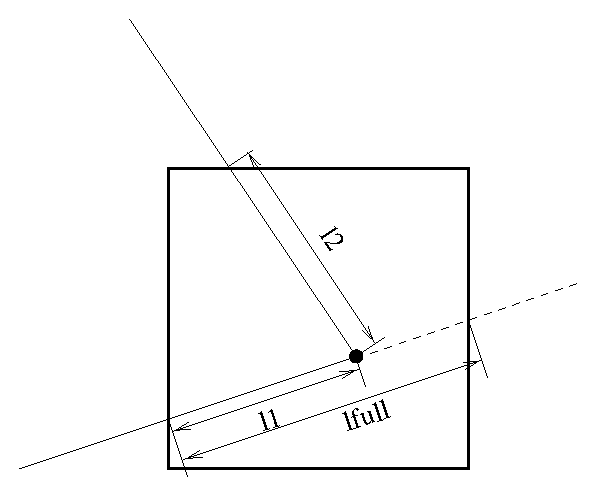
\includegraphics[width=0.6\textwidth]{figures/scatter.eps}
  \end{center}
\caption{The geometry of a scattering event within a powder sample.}
\label{powderFig}
\end{figure}

The probability for a given x-ray to be scattered from within the interval
$[ l_1 ; l_1+dl ]$ will be
\begin{equation}
P(l_1) dl = \mu^s f_\mathrm{att}(l_1) dl ,
\end{equation}
while the probability for a x-ray to be scattered from within
this interval into the solid angle $\Omega$ {\em and}
not being scattered further
or absorbed on the way out of the sample is
\begin{equation}
P(l_1,\Omega) dl d\Omega =
  \mu^s f_\mathrm{att}(l_1) f_\mathrm{att}(l_2) \gamma(\Omega) d\Omega dl ,
\end{equation}
where $\gamma(\Omega)$ is the directional distribution
of the scattered x-rays, and $l_2$ is determined by
Monte Carlo chocies of $l_1$, $\Omega$,
and from the sample geometry, see e.g. figure \ref{powderFig}.

In our Monte-Carlo simulations, we may choose the scattering
parameters by making a Monte-Carlo choice of $l_1$ and $\Omega$
from a distribution different from $P(l_1,\Omega)$.
By doing this, we must adjust $\pi_i$ according to
the probability transformation rule (\ref{probrule}).
If we {\em e.g.}\ choose the scattering depth, $l_1$,
from a flat distribution in $[ 0 ; l_\mathrm{full} ]$,
and choose the directional dependence from $g(\Omega)$,
we have a Monte Carlo probability
\begin{equation}
f(l_1,\Omega) = g(\Omega) / l_\mathrm{full} ,
\end{equation}
$l_\mathrm{full}$ is here the path length through the sample
as taken by a non-scattered x-ray (although we here
assume that all simulated x-rays are being scattered).
According to (\ref{probrule}), the x-ray weight factor
is now adjusted by the amount
\begin{equation}     \label{sampleprob}
\pi_i(l_1,\Omega) =
 \mu^s l_\mathrm{full} \exp \left[ - (l_1+l_2) (\mu^a + \mu^s) \right]
  \frac{\gamma(\Omega)}{g(\Omega)} .
\end{equation}

In analogy with the source components, it is possible to define
"interesting" directions for the scattering.
One will then try to focus the scattered x-rays,
choosing a $g(\Omega)$, which peaks around these directions.
To do this, one uses (\ref{sampleprob}), where the
fraction $\gamma(\Omega)/g(\Omega)$ corrects for the focusing.
One must choose a proper distribution so that
$g(\Omega) > 0$ in every interesting direction. If this is not the
case, the Monte Carlo simulation gives incorrect results.
All samples have been constructed with a focusing
and a non-focusing option.


\subsection{Future development of sample components}
There is still room for much more development of functionality in
\MCX\ samples.

%\section{V\_sample: An incoherent scatterer, the V-sample}
\label{s:v_sample}
\index{Samples!Incoherent isotropic scatterer (Vanadium)}
\index{Incoherent elastic scattering}

\component{V\_sample}{System}{$r_{\rm i}$, $r_{\rm o}$, $h$, $r_{\rm foc}$, $x_{\rm target}$, $y_{\rm target}$, $z_{\rm target}$}{$w_x$, $h_y$, $t_z$, $w_{\rm focus}, h_{\rm focus}$, $w_{\rm foc, angle}$, $h_{\rm foc, angle}$, \\ $\sigma_{\rm abs}$, $\sigma_{\rm inc}$, $V_0$, $f_{\rm pack}$, target\_index}{validated}

A sample with incoherent scattering, e.g. vanadium, is frequently used for
calibration purposes, as this gives an isotropic, elastically scattered beam.

The component {\bf V\_sample}
has {\em only} absorption and incoherent elastic scattering.
For the sample geometry, we default use a
hollow cylinder (which has the solid cylinder as a limiting case).
The sample dimensions are: Inner radius $r_{\rm i}$,
outer radius $r_{\rm o}$, and height $h$, see figure \ref{f:v-sample}.
\begin{figure}
  \begin{center}
    \psfrag{ri}{$r_i$}
    \psfrag{ro}{$r_o$}
    \psfrag{h}{$h$}
    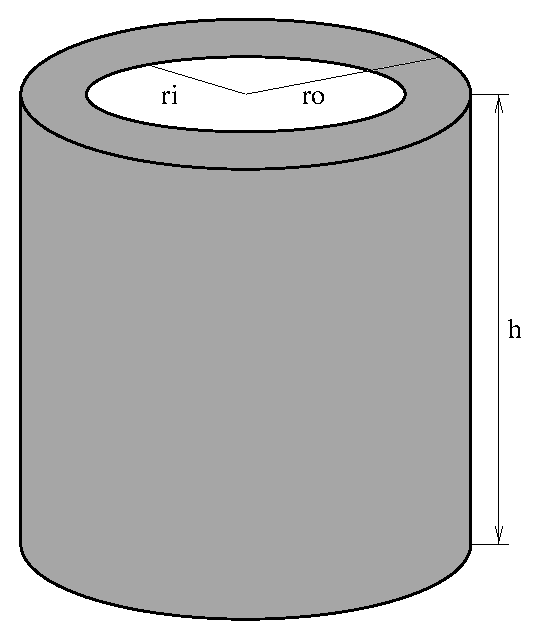
\includegraphics[width=0.3\textwidth]{figures/vsample.eps}
  \end{center}
\caption{The geometry of the hollow-cylinder vanadium sample.}
\label{f:v-sample}
\end{figure}

Alternatively, the sample geometry can be made rectangular
by specifying the width, $w_x$, the height, $h_y$, and the thickness, $t_z$.

The incoherent and absorption cross sections for V are default
for the component. For other choices, the
parameters $\sigma_{\rm inc}$, $\sigma_{\rm abs}$,
and the unit cell volume $V_0$ should be specified.
For a loosely packed sample, also the packing factor, $f_{\rm pack}$
can be specified (default value of 1).

\subsection{Physics and algorithm}

The incoherent scattering gives
a uniform angular distribution of the scattered
neutrons from each nucleus: $\gamma(\Omega) = 1/4\pi$.
For the focusing we choose to have a uniform distribution on
a target sphere of radius $r_{\rm foc}$, at the position
$(x_{\rm target},y_{\rm target},z_{\rm target})$
in the local coordinate system.
This gives an angular distribution (in a small angle approximation)
of
\begin{equation}
g(\Omega) = \frac{1}{4\pi}
  \frac{x_{\rm t}^2+y_{\rm t}^2+z_{\rm t}^2}{(\pi r_{\rm t}^2)}.
\end{equation}

The focusing can alternatively be performed on a rectangle with dimensions
$w_{\rm focus}$, $h_{\rm focus}$, or uniformly in angular space
(in a small-angle approximation),
using $w_{\rm foc, angle}$, $h_{\rm foc, angle}$.
The focusing location can be picked to be a downstream component by
specifying \\
\verb+target_index+.

When calculating the neutron path length within
the cylinder, the kernel function \\
\verb+cylinder_intersect+
is used twice, once for the outer radius and once
for the inner radius.

Multiple scattering is not included in this component. To obtain
intensities similar to real measured ones, we therefore do not
take attenuation from scattering into account for the outgoing
neutron ray.

\subsection{Remark on functionality}
When simulating a realistic incoherent hollow cylinder sample
one finds that  the resulting direction dependence
of the scattered intensity is {\em not} isotropic.
This is explained by the variation of attenuation with
scattering angle.
One test result is shown in the instrument example chapter of the \MCS\ User Manual.

The \verb+Samples_vanadium+ and \verb+Samples_incoherent+ test/example instruments exist in the distribution for this component.
         \newpage
%\section{Tunneling\_sample: An incoherent inelastic scatterer}
\label{s:Tunneling_sample}
\index{Samples!Incoherent inelastic scatterer}
\index{Incoherent inelastic scattering}

\component{Tunneling\_sample}{System}{$r_{\rm i}$, $r_{\rm o}$, $h$, $r_{\rm foc}$, $x_{\rm target}$, $y_{\rm target}$, $z_{\rm target}$}{$w_x$, $h_y$, $t_z$, $w_{\rm focus}, h_{\rm focus}$, $w_{\rm foc, angle}$, $h_{\rm foc, angle}$, $\sigma_{\rm abs}$, $\sigma_{\rm inc}$, $V_0$, $f_{\rm pack}$, $f_{\rm QE}$, $f_{\rm tun}$, $\Gamma$, $E_{\rm tun}$, target\_index}{not validated}

The component {\bf Tunneling\_sample}
displays incoherent inelastic scattering as found in a number of systems, {\em e.g.}
containing mobile hydrogen. 

For the sample geometry, we default use a
hollow cylinder (which has the solid cylinder as a limiting case).
The sample dimensions are: Inner radius $r_{\rm i}$,
outer radius $r_{\rm o}$, and height $h$. This geometry is the same as 
the default for {\bf V\_sample}, see figure \ref{f:v-sample}.

As for {\bf V\_sample}, the sample geometry can be made rectangular 
by specifying the width, $w_x$, the height, $h_y$, and the thickness, $t_z$.

Also the focusing properties are the same as for {\bf V\_sample}.
For the focusing is performed as a uniform distribution on
a target sphere of radius $r_{\rm foc}$, at the position
$(x_{\rm target},y_{\rm target},z_{\rm target})$
in the local coordinate system.
The focusing can alternatively be performed on a rectangle with dimensions
$w_{\rm focus}$, $h_{\rm focus}$, or uniformly in angular space
(in a small-angle approximation),
using $w_{\rm foc, angle}$, $h_{\rm foc, angle}$.
The focusing location can be picked to be a downstream component by
specifying \verb+target_index+.

The incoherent and absorption cross sections for V are default
for the component. For other choices, the
parameters $\sigma_{\rm inc}$, $\sigma_{\rm abs}$,
and the unit cell volume $V_0$ should be specified.
For a loosely packed sample, also the packing factor, $f_{\rm pack}$
can be specified (default value of 1).

The inelastic scattering takes place as a quasielastic (Lorentzian)
component, which is chosen with probability $f_{\rm QE}$.
The broadening of the signal is given by $\Gamma$ (HWHM).
In addition, a tunneling signal is present with a probability of $f_{\rm tun}$ 
and a tunneling energy of $\pm E_{\rm tun}$. 
The tunneling peaks are weighted by the usual factor $k_{\rm f}/k_{\rm i}$.

The total scattering cross section is given by
\begin{eqnarray}
\lefteqn{\frac{d^2\sigma}{d\Omega dE_{\rm f}}(q,\omega) = \frac{\sigma_{\rm inc}}{4\pi}
\times \left\{ (1-f_{\rm QE}-f_{\rm inel}) \delta(\hbar \omega) \right. }  \\
 &+& f_{\rm QE} \frac{\Gamma}{(\hbar\omega)^2+\Gamma^2}
 + \left.\frac{f_{\rm inel}}{2} \frac{k_{\rm f}}{f_{\rm i}} 
   \left[\delta(\hbar\omega-E_{\rm tun}) + \delta(\hbar\omega+E_{\rm tun}) \right] \right\} \nonumber
\end{eqnarray}

The component takes care that 
$f_{\rm QE} + f_{\rm tun} \leq 1$, otherwise an error is returned.

The component accounts for absorption, 
but not multiple scattering. To obtain
intensities similar to real measured ones, we therefore do not 
take attenuation from scattering into account for the outgoing
neutron ray.

        \newpage
\section{Absorption\_sample: An absorption phantom}
\index{Samples!Absorption}
\index{Tomography}
\label{absorption_sample}
\mcdoccomp{samples/Absorption_sample.parms}

This component models an absorption phantom with a single inclusion in surrounding material. It is intended use
is for tomographic imaging simulations.

%describe data format
 
\newpage
\section{Saxs\_spheres: A model of dilute hard spheres in solution for SAXS-use}
\index{Samples!SAXS}
\index{Samples!Dilute colloid medium}
\index{Diffraction}
\index{Small angle scattering}
\label{saxs_spheres}

\mcdoccomp{samples/Saxs_spheres.parms}

%The component {\bfseries Sans\_spheres} models a sample of small independent
%spheres of radius $R$, which are uniformly distributed
%in a rectangular volume $x_w \times y_h \times z_t$ with a volume
%fraction $\phi$. The absorption cross section density for the spheres
%is $\sigma_a$ (in units of m$^{-1}$), specified
%for neutrons at 2200 m/s. Absorption and incoherent scattering
%from the medium is neglected.
%The difference in scattering length density
%(the contrast) between the hard spheres and the medium is called $\Delta \rho$.
%$d$ denotes the distance to the (presumed circular) SANS detector of radius $R$.
%
%A usage example of this component can be found in the \verb+Neutron site/tests/SANS+ instrument from the \verb+mcgui+.
%
%\subsection{Small-angle scattering cross section}
%The neutron intensity scattered into a solid angle $\Delta \Omega$
%for a flat isotropic SANS sample in transmission geometry
%is given by \cite{ILLblue}:
%\begin{equation}
%I_s(q) = \Psi \Delta\Omega T A z_\mathrm{max} \frac{d\sigma_v}{d\Omega}(q) ,
%\end{equation}
%where $\Psi$ is the neutron flux, $T$ is the sample transmission,
%$A$ is the illuminated sample area, and $z_\mathrm{max}$ the length of
%the neutron path through the sample.
%
%In this component, we consider only scattering from a thin solution
%of monodisperse hard spheres of radius $R$, where the volume-specific
%scattering cross section is given by \cite{ILLblue}
%\begin{equation}
%\frac{d\sigma_v}{d\Omega}(q) =
%  n (\Delta\rho)^2 V^2 f(q)  ,
%\end{equation}
%where $f(q) = \left( 3\frac{\sin(qR)-qR\cos(qR)}{(qR)^3} \right)^2$,
%$n$ is the number density of spheres, and $V = 4 / 3 \pi R^3$ is the
%sphere volume. (The density is thus $n = \phi/V$.)
%
%Multiple scattering is ignored.
%
%\subsection{Algorithm}
%All neutrons, which hit the sample volume, are scattered.
%(Hence, no direct beam is simulated.)
%For scattered neutrons, the following steps are taken:
%\begin{enumerate}
%\item Choose a value of $q$ uniformly in the interval $[0;q_\mathrm{max}]$.
%\item Choose a polar angle, $\alpha$,
%  for the {\bfseries q}-vector uniformly in $[0;\pi]$.
%\item Scatter the neutron according to $(q,\alpha)$.
%\item Calculate and apply the correct weight factor correction.
%\end{enumerate}
%
%\subsection{Calculating the weight factor}
%The scattering position is found by a Monte Carlo choice uniformly
%along the whole (unscattered) beam path with the sample, length $l_\mathrm{full}$, giving
%$f_l = 1/l_\mathrm{full}$. The direction focusing on the detector gives
%(in an small angle approximation) $f_\Omega = d^2 / (\pi R_\mathrm{det}^2)$.
%
%Hence, the total weight tranformation factor becomes % (more explanation to come)
%\begin{equation}
%\pi_j = l_\mathrm{full} (\pi R_\mathrm{det}^2 / d^2)/(4 \pi)
%  n (\Delta\rho)^2 V^2 f(q) \exp(-\mu_a l) ,
%\end{equation}
%where $\mu_a$ is the linear attenuation factor due to absorption
%and $l$ is the total neutron path length within the sample.
%
%This component does NOT simulate absolute intensities. This latter depends on the detector parameters. \index{Bugs}
%
%Some alternative implementations exist as contributed components.
%
%The \verb+SANS+ test/example instrument exists in the distribution for this component.
 \newpage
\section{PowderN: A general powder sample}
\index{Samples!Powder, multiple diffraction line}
\index{Diffraction}
\index{Sample environments}
\index{Concentric components}
\label{powder}

\component{Powder\_N}{System}{$radius$, $thickness$, $h$, $xwidth$, $yheight$, $zdepth$, $\sigma_{\rm abs}$,
  $\sigma_{\rm inc}$, $Vc$, $f_{\rm pack}$, reflections, format, DW, concentic, and more}{}{}

The powder diffraction component {\bf PowderN} models a powder sample
with background coming only from incoherent scattering and no
multiple scattering. At the users choice, a given percentage of the incoming
events may be transmitted (attenuated) to model the direct beam. The component can also
assume \emph{concentric} shape, i.e. be used for describing sample environment (cryostat,
sample container etc.). 

The description of the powder comes from a file in one of the standard output formats LAZY, FULLPROF, or CRYSTALLOGRAPHICA.

A usage example of this component can be found in the \\
\verb+Neutron site/Tutorial/templateDIFF+ instrument from the \verb+mcgui+.

\subsection{Files formats: powder structures}

Data files of type \verb'lau' and \verb'laz' in the \MCS distribution data directory are self-documented in their header. A list of common powder definition files is available in Table \ref{t:powders-data} (page \pageref{t:powders-data}). They do not need any additional parameters to be used, as in the example:
\begin{lstlisting}
  PowderN(<geometry parameters>, filename="Al.laz")
\end{lstlisting}
Other column-based file formats may also be imported e.g. with parameters such as:
\begin{lstlisting}
  format=Crystallographica
  format=Fullprof
  format={1,2,3,4,0,0,0,0}
\end{lstlisting}
In the latter case, the indices define order of columns parameters
multiplicity, lattice spacing, $F^2$, Debye-Waller factor and intrinsic line width.

The column signification may as well explicitely be set in the data file header using any of the lines:
\begin{lstlisting}
  #column_j     <index of the multiplicity 'j' column>
  #column_d     <index of the d-spacing 'd' column>
  #column_F2    <index of the squared str. factor '|F|^2' column [b]>
  #column_F     <index of the structure factor norm '|F|' column>
  #column_DW    <index of the Debye-Waller factor 'DW' column>
  #column_Dd    <index of the relative line width Delta_d/d 'Dd' column>
  #column_inv2d <index of the 1/2d=sin(theta)/lambda 'inv2d' column>
  #column_q     <index of the scattering wavevector 'q' column>
\end{lstlisting}

Other component parameters may as well be specified in the data file
header with lines e.g.:
\begin{lstlisting}
  #V_rho        <value of atom number density [at/Angs^3]>
  #Vc           <value of unit cell volume Vc [Angs^3]>
  #sigma_abs    <value of Absorption cross section [barns]>
  #sigma_inc    <value of Incoherent cross section [barns]>
  #Debye_Waller <value of Debye-Waller factor DW>
  #Delta_d/d    <value of Detla_d/d width for all lines>
  #density      <value of material density [g/cm^3]>
  #weight       <value of material molar weight [g/mol]>
  #nb_atoms     <value of number of atoms per unit cell>
\end{lstlisting}

Further details on file formats are available in the \verb+mcdoc+ page
of the component.

\subsection{Geometry, physical properties, concentricity}
The sample has the shape of a solid cylinder, radius $r$ and height $h$ or a box-shaped
sample of size $xwidth$ x $yheight$ x $zdepth$. At the users choice, an inner 'hollow' can be
specified using the parameter $thickness$. 


As the Isotropic\_Sqw component~\ref{s:isotropic-sqw}, PowderN assumes \emph{concentric} shape, i.e.
can contain other components inside the inner hollow. To allow this, two almost identical copies
of the PowderN components must be set up \emph{around} the internal component(s), for example:


\begin{lstlisting}
COMPONENT Cryo = PowderN(reflections="Al.laz", radius = 0.01, thickness = 0.001,
                          concentric = 1)
AT (0,0,0) RELATIVE Somewhere

COMPONENT Sample = some_other_component(with geometry FULLY enclosed in the hollow)
AT (0,0,0) RELATIVE Somewhere

COMPONENT Cryo2 = COPY(Cryo)(concentric = 0)
AT (0,0,0) RELATIVE Somewhere
\end{lstlisting}

As outlined, the first instance of PowderN \emph{must} have \verb+concentric = 1+ and the instance \emph{must}
have \verb+concentric = 0+. Furthermore, the component(s) inside the hollow \emph{must} have a geometry which can
be fully contained inside the hollow.


In addition to the coherent scattering specified in the \verb+reflections+ file, absorption- and incoherent 
cross sections can be given using the input parameters $\sigma_c^a$ and $\sigma_i^s$.


The Bragg scattering from the powder,
$\sigma_c^s$ is calculated from the input file, with the parameters
$Q$, $|F(Q)|^2$, and $j$ for the scattering vector, structure factor, and
multiplicity, respectively. The volume of the unit cell is denoted $Vc$,
while the sample packing factor is $f_{\rm pack}$.


%Further, the incoherent scattering is only taken into account
%by the attenuation of the beam, given by (\ref{e:attenu})
%and $\sigma_c^a$.
%The incoherently scattered neutrons are not
%propagated through to the detector, but rather not generated at all.

Focusing is performed by only scattering into one angular
interval, $d\phi$ of the Debye-Scherrer circle. The center of this
interval is located at the point where the Debye-Scherrer circle
intersects the half-plane defined by the initial velocity, ${\bf v}_{\rm i}$,
and a user-specified vector, {\bf f}.

%The input parameters for this component are
%
%\begin{lstlisting}\begin{tabular}{ccl}
%$r$ & m & Radius of cylinder \\
%$h$ & m & Height of cylinder \\
%$\sigma_c^a$ & fm$^2$ & Absorption cross section per unit cell (at 2200 m/s) \\
%$\sigma_{i,c}^s$ & (fm)$^2$ & Incoherent scattering cross section per unit cell \\
%$\rho'/\rho$ & 1 & Packing factor \\
%$V_c$ & \AA$^3$ & Volume of unit cell \\
%${\bf Q}$ & \AA$^{-1}$ & The reciprocal lattice vector under consideration \\
%$|F({\bf Q}_j)|^2$ & (fm)$^2$ &
% Structure factor \\
%$j$ & 1 & Multiplicity of reflection \\
%$\exp(-2W)$ & 1 & Debye-Waller factor \\
%$d\phi$ & deg & Angular interval of focusing \\
%$f_x$ & m & \\
%$f_y$ & m & Focusing vector\\
%$f_z$ & m & \\
%\end{tabular}\end{lstlisting}

\subsection{Powder scattering}
An ideal powder sample consists of many small
crystallites, although each crystallite is sufficiently
large not to cause measurable size broadening.
The orientation of the crystallites is evenly distributed,
and there is thus always a large number of
crystallites oriented to fulfill the Bragg condition
\begin{equation}   \label{Bragg}
n \lambda = 2 d \sin \theta ,
\end{equation}
where $n$ is the order of the scattering (an integer), $\lambda$
is the neutron wavelength, $d$ is the lattice spacing of the sample,
and $2 \theta$ is the scattering angle, see figure \ref{coneFig}.
As all crystal orientations
are realised in a powder sample, the neutrons are scattered within a
{\em Debye-Scherrer cone} of opening angle $4 \theta$ \cite{bacon}.

\begin{figure}
  \begin{center}
    \psfrag{2theta}[c][c]{$2\theta$}
    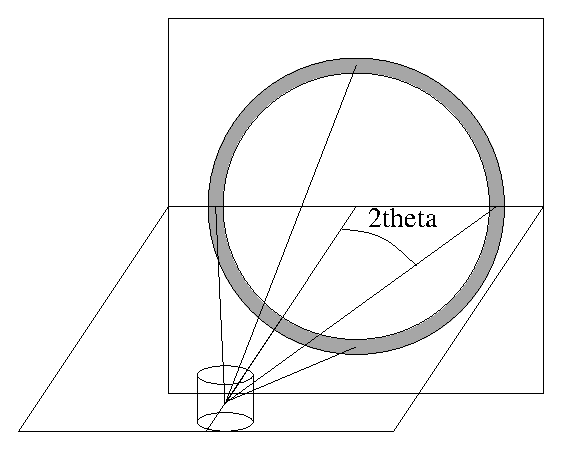
\includegraphics[width=0.6\textwidth]{figures/powder}
  \end{center}
\caption{The scattering geometry of a powder sample showing part of the
Debye-Scherrer cone (solid lines) and the Debye-Scherrer circle (grey).}
\label{coneFig}
\end{figure}

Equation (\ref{Bragg}) may be cast into the form
\begin{equation}
|{\bf Q}| = 2 |{\bf k}| \sin \theta ,
\end{equation}
where {\bf Q} is a vector of the reciprocal lattice, and {\bf k} is
the wave vector of the neutron. It is seen that only
reciprocal vectors fulfilling $|{\bf Q}| < 2 |{\bf k}|$
contribute to the scattering.
For a complete treatment of the powder sample, one needs to take
into account all these {\bf Q}-values, since each of them contribute
to the attenuation.

The strength of the Bragg reflections is given by their structure factors
\begin{equation}
 \left| \sum_j b_j \exp({\bf R}_j \cdot {\bf Q}) \right|^2 ,
\end{equation}
where the sum runs over all atoms in one unit cell. This structure factor is
non-zero only when $Q$ equals a reciprocal lattice vector.

The textbook expression for the scattering cross section
corresponding to one Debye-Scherrer cone reads \cite[ch.3.6]{squires}, with $V=N V_0$ being the total sample volume:
\begin{equation}
\sigma_{\rm cone}
  = \frac{V}{V_0^2} \frac{\lambda^3}{4 \sin \theta} \sum_Q |F(Q)|^2 .
\end{equation}
For our purpose, this expression should be changed slightly.
Firstly, the sum over structure factors for a particular $Q$ is replaced
by the sum over essentially different reflections multiplied by their
multiplicity, $j$. Then, a finite packing factor, $f$, is defined for the powder,
and finally, the Debye-Waller factor is multiplied on the elastic cross section
to take lattice vibrations into account (no inelastic background is simulated,
however). We then reach
\begin{eqnarray}
\sigma_{\rm cone, Q}
 & = & j_Q f \exp(-2W) \frac{V}{V_0^2} \frac{\lambda^3}{4 \sin \theta} |F(Q)|^2 \\
 & = & f \exp(-2W) \frac{N}{V_0} \frac{4\pi^3}{k^2} \frac{j_Q |F(Q)|^2}{Q}
\end{eqnarray}
in the thin sample approximation. For samples of finite thickness, the
beam is being attenuated by the attenuation coefficient
\begin{equation}
\label{e:attenu}
\mu_{\rm Q} = \sigma_{\rm cone,Q} / V .
\end{equation}
For calibration it may be useful to consider the total intensity
scattered into a detector of effective height $h$, covering only
one reflection \cite[ch.3.6]{squires}.
A cut though the Debye-Scherrer cone perpendicular to its axis
is a circle. At the distance $r$ from the sample, the radius of this
circle is $r \sin(2\theta)$. Thus, the detector (in a small angle
approximation) counts a fraction $h / (2 \pi r \sin(2 \theta))$
of the scattered neutrons, giving a resulting count intensity:
\begin{equation}
I = \Psi \sigma_{\rm cone,Q} \frac{h}{2 \pi r \sin(2\theta)} ,
\end{equation}
where $\Psi$ is the flux at the sample position.

For clarity we repeat the meaning and unit of the symbols:
%
\begin{lstlisting}
\begin{tabular}{ccl}
$\Psi$ & s$^{-1}$m$^{-2}$ & Incoming intensity of neutrons \\
$I$    & s$^{-1}$ & Detected intensity of neutrons \\
$h$    & m        & Height of detector \\
$r$    & m        & Distance from sample to detector \\
$f$    & 1        & Packing factor of the powder \\
$j$    & 1        & Multiplicity of the reflection \\
$V_0$  & m$^{3}$  & Volume of unit cell\\
$|F({\bf Q})|^2$ & m$^2$  & Structure factor \\
$\exp(-2W)$ & 1  & Debye-Waller factor \\
$\mu_{\rm Q}$ & m$^{-1}$ & Linear attenuation factor due to scattering from
one powder line. \\
\end{tabular}
\end{lstlisting}
%
%Often, one defines the {\em scattering power} as
%\begin{equation}
%Q \equiv N^2 \frac{|F({\bf Q})|^2 \lambda^3}{V \sin(2\theta)}
% = N_c^2 V \frac{\rho'}{\rho} \frac{|F({\bf Q})|^2 \lambda^3}{\sin(2\theta)} ,
%\end{equation}
%where $N$ is the number of unit cells.

A powder sample will in general have several allowed reflections
${\bf Q}_j$, which will all contribute to the attenuation.
These reflections will have different values of
$|F({\bf Q}_j)|^2$ (and hence of $Q_j$), $j_j$, $\exp(-2W_j)$,
and $\theta_j$.
The total attenuation through the sample due to scattering is given by
$\mu^s = \mu_{\rm inc}^s + \sum_j \mu^s_j $,
where $\mu_{\rm inc}^s$ represents the incoherent scattering.

\subsection{Algorithm}
The algorithm of {\bf PowderN} can be summarized as
\begin{itemize}
\item Check if the neutron ray intersects the sample (otherwise ignore
the following).
\item Calculate the attenuation coefficients for scattering and absorption.
\item Perform Monte Carlo choices to determine the scattering position,
scattering type (coherent/incoherent), and the outgoing direction.
\item Perform the necessary weight factor transformation.
\end{itemize}

%\subsection{Calculating the weight factor}
          \newpage
\section{Perfect\_crystal: A Darwin-width domniated single crystal model}

\index{Samples!single crystal, darwin}
\label{perfect_crystal}
\mcdoccomp{samples/Perfect_crystal.parms}

Pedning Further Documetation
\newpage
\section{Single\_crystal: The single crystal component}
\label{s:Single_crystal}
\index{Samples!Single crystal diffraction}
\index{Diffraction}
\index{Incoherent elastic scattering}
\index{Multiple scattering}

\component{Single\_crystal}{Kristian Nielsen}{$x_{width}, y_{height}, z_{thick}$,$\vec a, \vec b, \vec c, \Delta d/d$, mosaic, reflections}{$\sigma_{abs}, \sigma_{inc}$, ...}{Partially validated, centered. Further validation undergoing. Known BUGS: The component is known not to work as a Bragg monochromator, likely the problem relates to the internal definition of the reciprocal space. Possibly related to this, the model of anistropic mosaic is broken - always use a non-zero isotropic mosaic. Also, always use a non-zero value of the $\Delta d/d$ parameter.}

The {\bf Single\_crystal} component models a thick, flat single crystal
with multiple scattering and absorption with elastic coherent scattering.
An elastic incoherent background may also be simulated.
It may be used to describe samples for diffraction,
but also for accurate monochromator descriptions.
The component is currently under further review. The current documentation is outdated, especially with respect to the model of crystal mosaicity.

The input parameters for the component are \textit{xwidth},
\textit{yheight}, and \textit{zdepth} to define the dimensions of the
crystal in meters (area is centered); \textit{delta\_d\_d} to give the
value of $\Delta d/d$ (no unit);
$(\textit{ax}, \textit{ay}, \textit{az})$, $(\textit{bx}, \textit{by},
\textit{bz})$, and $(\textit{cx}, \textit{cy}, \textit{cz})$ to define
the axes of the direct lattice of the crystal (the sides of the unit
cell) in units of {\AA}ngstr{\o}m; and \textit{reflections}, a string
giving the name of the file with the list of structure factors to
consider.
The mosaic is specified \emph{either} isotropically as
\textit{mosaic}, \emph{or} anisotropically as \textit{mosaic\_h}
(rotation around the $Y$ axis), \textit{mosaic\_v} (rotation around the
$Z$ axis), and \textit{mosaic\_n} (rotation around the $X$ axis); in all
cases in units of full-width-half-maximum minutes of arc.

Optionally, the absorption cross-section at 2200 m/s and the incoherent
cross-section may be given as \textit{absorption} and
\textit{incoherent} (in barns), with default of zero; and
\textit{p\_transmit} may be assigned a fixed Monte Carlo probability for
transmission through the crystal without any interaction.

The user must specify a list of reciprocal lattice vectors
$\boldsymbol{\tau}$ to consider along with their structure factors
$|F_{\boldsymbol{\tau}}|^2$. The user must also specify the coordinates
(in direct space) of the unit cell axes $\boldsymbol{a}$,
$\boldsymbol{b}$, and $\boldsymbol{c}$, from which the reciprocal lattice
will be computed. See section \ref{s:Single_crystal_implement} for file format specifications.

In addition to coherent scattering, {\bf Single\_crystal} also
handles incoherent scattering and absorption. The incoherent scattering
cross-section is supplied by the user as a constant
$\sigma_{\rm inc}$. The absorption cross-section is supplied by the user at
2200~m/s, so the actual cross-section for a neutron of velocity $v$ is
$\sigma_{\rm abs} = \sigma_{2200} \frac{\rm 2200~m/s}{v}$.

\subsection{The physical model}

The textbook expression for the scattering cross-section of a crystal
is~\cite[ch.3]{squires}:
\begin{equation}
\label{eq:sigma_coh_el}
\left(\frac{d\sigma}{d\Omega}\right)_{\rm coh.el.} =
        N\frac{(2\pi)^3}{V_0}\sum_{\boldsymbol{\tau}}
        \delta(\boldsymbol{\tau} - \boldsymbol{\kappa})|F_{\boldsymbol{\tau}}|^2
\end{equation}
Here $|F_{\boldsymbol{\tau}}|^2$ is the structure factor
(defined in section~\ref{powder}), $N$ is the
number of unit cells, $V_0$ is the volume of an
individual unit cell, and $\boldsymbol{\kappa} (= {\bf k}_i - {\bf k}_f)$
is the scattering vector. $\delta(\boldsymbol{x})$ is a 3-dimensional delta
function in reciprocal space,
so for given incoming wave vector ${\bf k}_i$ and lattice vector
${\boldsymbol{\tau}}$, only a single final wave vector ${\bf k}_f$ is allowed.
In general, this wavevector will not fulfill the conditions for elastic
scattering $(k_f = k_i)$.
In a real crystal, however, reflections are not perfectly sharp. Because
of imperfection and finite-size effects, there will be a small region
around $\boldsymbol{\tau}$ in reciprocal space of possible scattering vectors.

{\bf Single\_crystal} simulates a crystal with a mosaic spread
$\eta$ and a lattice plane spacing uncertainty $\Delta d/d$. In such
crystals the reflections will not be completely sharp;
there will be a small region around each reciprocal lattice point of the
crystal that contains valid scattering vectors.

We model the mosaicity and $\Delta d/d$ of the crystal with
3-dimensional Gaussian functions in reciprocal space (see
figure~\ref{fig:crystal-reciprocal-space}). Two of the axes of the
Gaussian are perpendicular to the reciprocal lattice vector $\boldsymbol{\tau}$ and model
the mosaicity. The third one is parallel to $\boldsymbol{\tau}$ and models
$\Delta d/d$. We assume that the
mosaicity is small so that the possible directions of the scattering
vector may be approximated with a Gaussian in rectangular
coordinates.
\begin{figure}[t]
  \begin{center}
    \psfrag{ki}[r][r]{$\boldsymbol{k}_{\rm i}$}
    \psfrag{kf}[l][l]{$\boldsymbol{k}_{\rm f}$}
    \psfrag{tau}[r][r]{$\boldsymbol{\tau}$}
    \psfrag{mosaic}[l][l]{$\eta$}
    \psfrag{del-d-d}[l][l]{$\Delta d/d$}
    \psfrag{Ewald}[l][l]{Ewald}
    \psfrag{Sphere}[l][l]{Sphere}
    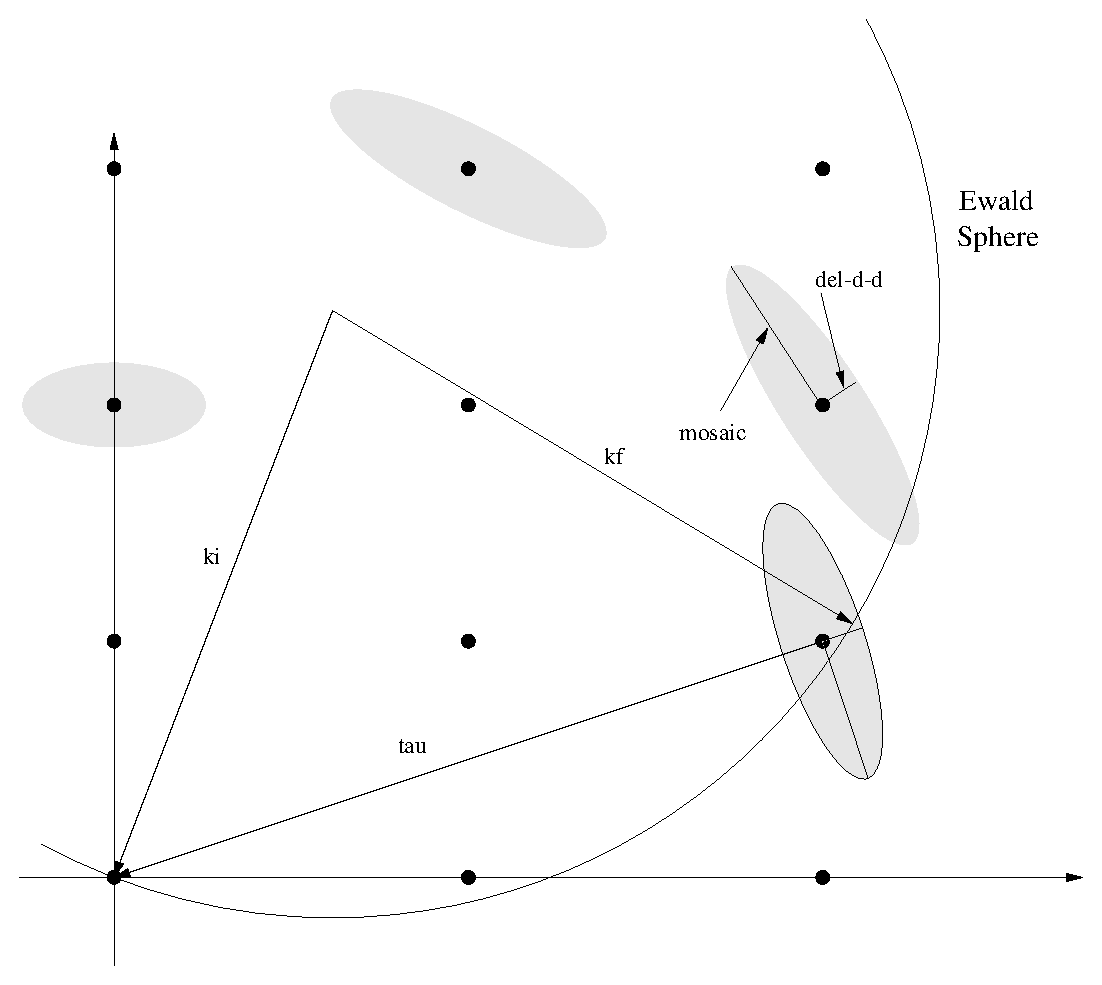
\includegraphics[width=0.7\textwidth]{figures/recip_space3.eps}
  \end{center}
\caption{Ewald sphere construction for a single neutron showing the
    Gaussian broadening of reciprocal lattice points in their local
    coordinate system.}
\label{fig:crystal-reciprocal-space}
\end{figure}

If the mosaic is isotropic (the same in all directions), the two
Gaussian axes perpendicular to $\boldsymbol{\tau}$ are simply arbitrary
normal vectors of equal length given by the mosaic. But if the mosaic
is anisotropic, the two perpendicular axes will in general be different
for each scattering vector. In the absence of anything better,
{\bf Single\_crystal} uses a model which is at least mathematically
plausible and which works as expected in the two common cases:
(1)~isotropic mosaic, and (2)~two mosaic directions (``horizontal and
vertical mosaic'') perpendicular to a scattering vector.

The basis for the model is a three-dimensional Gaussian distribution in
Euler angles giving the orientation probability distribution for the
micro-crystals; that is, the misorientation is given by small rotations
around the $X$, $Y$, and $Z$ axes, with the rotation angles having (in
general different) Gaussian probability distributions. For given
scattering vector $\boldsymbol{\tau}$, a rotation of the micro-crystals
around an axis parallel to $\boldsymbol{\tau}$ has no effect on the
direction of the scattering vector. Suppose we form the intersection
between the three-dimensional Gaussian in Euler angles and a plane
through the origin perpendicular to $\boldsymbol{\tau}$. This gives a
two-dimensional Gaussian, say with axes defined by unit vectors
$\boldsymbol{g}_1$ and $\boldsymbol{g}_2$ and mosaic widths $\eta_1$ and
$\eta_2$.

We now let the mosaic for $\boldsymbol{\tau}$ be defined by rotations
around $\boldsymbol{g}_1$ and $\boldsymbol{g}_2$ with angles having
Gaussian distributions of widths $\eta_1$ and $\eta_2$. Since
$\boldsymbol{g}_1$, $\boldsymbol{g}_2$, and $\boldsymbol{\tau}$ are
perpendicular, a small rotation of $\boldsymbol{\tau}$ around
$\boldsymbol{g}_1$ will change $\boldsymbol{\tau}$ in the direction of
$\boldsymbol{g}_2$. The two axes of the Gaussian mosaic in reciprocal
space that are perpendicular to $\boldsymbol{\tau}$ will thus be given
by $\tau\eta_2\boldsymbol{g}_1$ and $\tau\eta_1\boldsymbol{g}_2$.

We now derive a quantitative expression for the scattering cross-section
of the crystal in the model. For this, we introduce a \emph{local
  coordinate system} for each reciprocal lattice point
$\boldsymbol{\tau}$ and use $\boldsymbol{x}$ for vectors written in local
coordinates. The origin is $\boldsymbol{\tau}$, the first axis
is parallel to $\boldsymbol{\tau}$ and the other two axes are
perpendicular to $\boldsymbol{\tau}$. In the local coordinate system,
the 3-dimensional Gaussian is given by
\begin{equation}
  \label{eq:crystal-gauss-1}
  G(x_1,x_2,x_3) = \frac{1}{(\sqrt{2\pi})^3}\frac{1}{\sigma_1\sigma_2\sigma_3}
  e^{-\frac{1}{2}(\frac{x_1^2}{\sigma_1^2} +
  \frac{x_2^2}{\sigma_2^2} + \frac{x_3^2}{\sigma_3^2})}
\end{equation}
The axes of the Gaussian are $\sigma_1 = \tau\Delta d/d$ and $\sigma_2 =
\sigma_3 = \eta\tau$. Here we used the assumption that $\eta$ is small,
so that $\tan\eta \approx \eta$ (with $\eta$ given in radians).  By
introducing the diagonal matrix
$$
D = \left(
  \begin{array}[c]{ccc}
    \frac{1}{2}\sigma_1^2 & 0 & 0 \\
    0 & \frac{1}{2}\sigma_2^2 & 0 \\
    0 & 0 & \frac{1}{2}\sigma_3^2
  \end{array}\right)
$$
equation~(\ref{eq:crystal-gauss-1}) can be written as
\begin{equation}
  G(\boldsymbol{x}) =
  \frac{1}{(\sqrt{2\pi})^3}\frac{1}{\sigma_1\sigma_2\sigma_3}
  e^{-\boldsymbol{x}^{\rm T} D \boldsymbol{x}}
\end{equation}
again with $\boldsymbol{x}=(x_1,x_2,x_3)$ written in local coordinates.

To get an expression in the coordinates of the reciprocal lattice of the
crystal, we introduce a matrix $U$ such that if $\boldsymbol{y} =
(y_1,y_2,y_3)$ are the global coordinates of a point in the crystal
reciprocal lattice, then $U(\boldsymbol{y} + \boldsymbol{\tau})$ are the
coordinates in the local coordinate system for $\boldsymbol{\tau}$. The
matrix $U$ is given by
$$ U^{\rm T} = (\hat{u}_1, \hat{u}_2, \hat{u}_3), $$
where $\hat{u}_1$, $\hat{u}_2$, and $\hat{u}_3$ are the axes of the
local coordinate system, written in the global coordinates of the
reciprocal lattice. Thus
$\hat{u}_1 = \boldsymbol{\tau}/\tau$,  and $\hat{u}_2$ and $\hat{u}_3$ are
unit vectors perpendicular to $\hat{u}_1$ and to each other.
The matrix $U$ is unitarian, that is
$U^{-1} = U^{\rm T}$. The translation between global and local
coordinates is
$$ \boldsymbol{x} = U(\boldsymbol{y} + \boldsymbol{\tau}) \qquad
   \boldsymbol{y} = U^{\rm T} \boldsymbol{x} - \boldsymbol{\tau} $$

The expression for the 3-dimensional Gaussian in global coordinates is
\begin{equation}
  G(\boldsymbol{y}) =
  \frac{1}{(\sqrt{2\pi})^3}\frac{1}{\sigma_1\sigma_2\sigma_3}
  e^{-(U(\boldsymbol{y}+\boldsymbol{\tau}))^{\rm T} D (U(\boldsymbol{y}+\boldsymbol{\tau}))}
\end{equation}
The elastic coherent cross-section is then given by
\begin{equation}
  \label{eq:crystal-cross-section}
  \left(\frac{d\sigma}{d\Omega}\right)_{\rm coh.el.} =
        N\frac{(2\pi)^3}{V_0}\sum_{\boldsymbol{\tau}}
        G(\boldsymbol{\tau} - \boldsymbol{\kappa})
         |F_{\boldsymbol{\tau}}|^2
\end{equation}

\subsection{The algorithm}

The overview of the algorithm used in the Single\_crystal component is
as follows:
\begin{enumerate}
\item\label{enum:crystal-1} Check if the neutron intersects the
  crystal. If not, no action is taken.
\item\label{enum:crystal-2} Search through a list of reciprocal lattice
  points of interest, selecting those that are close enough to the Ewald
  sphere to have a non-vanishing scattering probability. From these,
  compute the total coherent cross-section $\sigma_{\rm coh}$ (see
  below), the absorption cross-section $\sigma_{\rm abs} = \sigma_{\rm
  2200} \frac{{\rm 2200~m/s}}{v}$, and the total cross-section
  $\sigma_{\rm tot} = \sigma_{\rm coh}+\sigma_{\rm inc}+\sigma_{\rm abs}$.
\item\label{enum:crystal-3} The transmission probability is
  $\exp(- \frac{\sigma_{\rm tot}}{V_0}\ell)$ where $\ell$ is the length of
  the flight path through the crystal. A Monte Carlo choice is
  performed to determine
  whether the neutron is transmitted. Optionally, the user may
  set a fixed Monte Carlo probability for the first scattering event,
  for example to boost the statistics for a weak reflection.
\item\label{enum:crystal-4} For non-transmission, the position at which
  the neutron will interact is selected from an exponential
  distribution. A Monte Carlo choice is made of whether to scatter
  coherently or incoherently. Absorption is treated by weight adjustment
  (see below).
\item\label{enum:crystal-5} For incoherent scattering, the outgoing wave
  vector $\boldsymbol{k}_{\rm f}$ is selected with a random direction.
\item\label{enum:crystal-6} For coherent scattering, a reciprocal
  lattice vector is selected by a Monte Carlo choice, and
  $\boldsymbol{k}_{\rm f}$ is found (see below).
\item\label{enum:crystal-7} Adjust the neutron weight as dictated by the
  Monte Carlo choices made.
\item\label{enum:crystal-8} Repeat from~(\ref{enum:crystal-2}) until the
  neutron is transmitted (to simulate multiple scattering).
\end{enumerate}

For point~\ref{enum:crystal-2}, the distance
\textit{dist} between a reciprocal lattice point and the Ewald sphere is
considered small enough to allow scattering if it is less than five
times the maximum axis of the Gaussian, $\textit{dist} \leq
5\max(\sigma_1,\sigma_2,\sigma_3)$.

\subsection{Choosing the outgoing wave vector}

The final wave vector $\boldsymbol{k}_{\rm f}$ must lie on the
intersection between the Ewald sphere and the Gaussian ellipsoid. Since
$\eta$ and $\Delta d/d$ are assumed small, the intersection can be
approximated with a plane tangential to the sphere, see
figure~\ref{fig:crystal-scattering-tri}. The tangential point is taken
to lie on the line between the center of the Ewald sphere
$-\boldsymbol{k}_{\rm i}$ and the reciprocal lattice point
$\boldsymbol{\tau}$. Since the radius of the Ewald sphere is $k_{\rm
  i}$, this point is
$$ \boldsymbol{o}=(k_{\rm i}/\rho - 1)\boldsymbol{\rho} - \boldsymbol{\tau} $$
where $\boldsymbol{\rho} = \boldsymbol{k}_{\rm i} - \boldsymbol{\tau}$.
\begin{figure}[t]
  \begin{center}
    \psfrag{ki}[r][r]{$\boldsymbol{k}_{\rm i}$}
    \psfrag{kf}[l][l]{$\boldsymbol{k}_{\rm f}$}
    \psfrag{rho}[r][r]{$\boldsymbol{\rho}$}
    \psfrag{tau}[r][r]{$\boldsymbol{\tau}$}
    \psfrag{x}[l][l]{$\boldsymbol{x}$}
    \psfrag{Ewald}[r][r]{Ewald}
    \psfrag{Sphere}[r][r]{Sphere}
    \psfrag{Tangential}[l][l]{Tangential}
    \psfrag{plane}[l][l]{plane}
    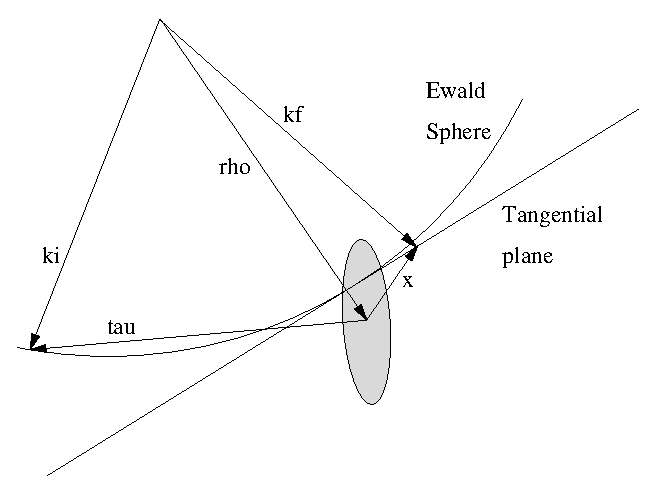
\includegraphics[width=0.7\textwidth]{figures/recip-detail.eps}
  \end{center}
\caption{The scattering triangle in the single crystal.}
\label{fig:crystal-scattering-tri}
\end{figure}

The equation for the plane is
\begin{equation}
  \label{eq:crystal-tangent-plane}
    \boldsymbol{P}(\boldsymbol{t}) = \boldsymbol{o} + B \boldsymbol{t}, \qquad
    \boldsymbol{t} \in \mathbb{R}^2
\end{equation}
Here $B = (\boldsymbol{b}_1, \boldsymbol{b}_2)$ is a $3\times 2$ matrix
with the two generators for the plane $\boldsymbol{b}_1$ and
$\boldsymbol{b}_2$. These are (arbitrary) unit vectors in the plane,
being perpendicular to
each other and to the plane normal $\boldsymbol{n} =
\boldsymbol{\rho}/\rho$.

Each $\boldsymbol{t}$ defines a potential final wave vector
$\boldsymbol{k}_{\rm f}(\boldsymbol{t}) = \boldsymbol{k}_{\rm i} +
\boldsymbol{P}(\boldsymbol{t})$. The value of the 3-dimensional Gaussian
for this $\boldsymbol{k}_{\rm f}$ is
\begin{equation}
  \label{eq:crystal-gauss-t-1}
  G(\boldsymbol{x}(\boldsymbol{t})) =
  \frac{1}{(\sqrt{2\pi})^3}\frac{1}{\sigma_1\sigma_2\sigma_3}
  e^{-\boldsymbol{x}(\boldsymbol{t})^{\rm T} D \boldsymbol{x}(\boldsymbol{t})}
\end{equation}
where $\boldsymbol{x}(\boldsymbol{t}) = \boldsymbol{\tau} -
(\boldsymbol{k}_{\rm i} - \boldsymbol{k}_{\rm f}(\boldsymbol{t}))$ is
given in local coordinates for $\boldsymbol{\tau}$. It can be shown that
equation~(\ref{eq:crystal-gauss-t-1}) can be re-written as
\begin{equation}
  \label{eq:crystal-gauss-2}
  G(\boldsymbol{x}(\boldsymbol{t})) =
  \frac{1}{(\sqrt{2\pi})^3}\frac{1}{\sigma_1\sigma_2\sigma_3} e^{-\alpha}
  e^{-(\boldsymbol{t}-\boldsymbol{t}_0)^{\rm T} M
    (\boldsymbol{t}-\boldsymbol{t}_0)}
\end{equation}
where $M = B^{\rm T} D B$ is a $2 \times 2$ symmetric and positive
definite matrix, $\boldsymbol{t}_0 = -M^{-1}B^{\rm T} D \boldsymbol{o}$
is a 2-vector, and $\alpha = -\boldsymbol{t}_0^{\rm T} M
\boldsymbol{t}_0 + \boldsymbol{o}^{\rm T} D \boldsymbol{o}$ is a real
number.  Note that this is a two-dimensional Gaussian (not necessarily
normalized) in $\boldsymbol{t}$ with center $\boldsymbol{t}_0$ and axis
defined by $M$.

To choose $\boldsymbol{k}_{\rm f}$ we sample $\boldsymbol{t}$ from the
2-dimensional Gaussian distribution~(\ref{eq:crystal-gauss-2}). To do
this, we first construct the Cholesky decomposition of the matrix
$(\frac{1}{2}M^{-1})$. This gives a $2\times 2$ matrix $L$ such that $L
L^{\rm T} = \frac{1}{2}M^{-1}$ and is possible since $M$ is symmetric
and positive definite. It is given by
$$
  L = \left(
  \begin{array}[c]{cc}
    \sqrt{\nu_{11}} & 0 \\
    \frac{\nu_{12}}{\sqrt{\nu_{11}}} & \sqrt{\nu_{22} - \frac{\nu_{12}^2}{\nu_{11}}}
  \end{array}\right)
\qquad\hbox{where }
  \frac{1}{2}M^{-1} = \left(
  \begin{array}[c]{cc}
    \nu_{11} & \nu_{12} \\
    \nu_{12} & \nu_{22}
  \end{array}\right)
$$
Now let $\boldsymbol{g} = (g_1, g_2)$ be two random numbers drawn form a
Gaussian distribution with mean 0 and standard deviation 1, and let
$\boldsymbol{t} = L\boldsymbol{g} + \boldsymbol{t}_0$. The probability
of a particular $\boldsymbol{t}$ is then
\begin{eqnarray}
  P(\boldsymbol{t})d\boldsymbol{t}
    &=& \frac{1}{2\pi}
      e^{-\frac{1}{2}\boldsymbol{g}^{\rm T}\boldsymbol{g}} d\boldsymbol{g} \\
    &=& \frac{1}{2\pi}\frac{1}{\det L}
      e^{-\frac{1}{2}(L^{-1}(\boldsymbol{t}-\boldsymbol{t}_0))^{\rm T}
          (L^{-1}(\boldsymbol{t}-\boldsymbol{t}_0))} d\boldsymbol{t} \\
    &=& \frac{1}{2\pi}\frac{1}{\det L}
      e^{-(\boldsymbol{t}-\boldsymbol{t}_0)^{\rm T}
          M(\boldsymbol{t}-\boldsymbol{t}_0)} d\boldsymbol{t}
  \label{eq:crystal-gauss-prob-1}
\end{eqnarray}
where we used that
$\boldsymbol{g}=L^{-1}(\boldsymbol{t}-\boldsymbol{t}_0)$ so that
$d\boldsymbol{g} = \frac{1}{\det L}d\boldsymbol{t}$. This is just the
normalized form of~(\ref{eq:crystal-gauss-2}). Finally we set
$\boldsymbol{k}'_{\rm f} = \boldsymbol{k}_{\rm i} +
\boldsymbol{P}(\boldsymbol{t})$ and
$\boldsymbol{k}_{\rm f} = (k_{\rm i}/k'_f)\boldsymbol{k}'_{\rm f}$ to
normalize the length of $\boldsymbol{k}_{\rm f}$ to correct for the
(small) error introduced by approximating the Ewald sphere with a plane.

\subsection{Computing the total coherent cross-section}

To determine the total coherent scattering cross-section, the differential
cross-section must be integrated over the Ewald sphere:
$$
\sigma_{\rm coh} = \int_{\rm Ewald}
\left(\frac{d\sigma}{d\Omega}\right)_{\rm coh.el.} d\Omega
$$
For small mosaic we may approximate the sphere with the tangential
plane, and we thus get from~(\ref{eq:crystal-cross-section})
and~(\ref{eq:crystal-gauss-2}):
\begin{eqnarray}
  \label{eq:crystal-coh-cs}
  \sigma_{{\rm coh},\boldsymbol{\tau}} &=& \int N\frac{(2\pi)^3}{V_0}
        G(\boldsymbol{\tau} - \boldsymbol{\kappa})
         |F_{\boldsymbol{\tau}}|^2 d\Omega \\
  &=& \frac{1}{\boldsymbol{k}_i^2} N\frac{(2\pi)^3}{V_0}
         \frac{1}{(\sqrt{2\pi})^3}\frac{e^{-\alpha}}{\sigma_1\sigma_2\sigma_3}
         |F_{\boldsymbol{\tau}}|^2
         \int e^{-(\boldsymbol{t}-\boldsymbol{t}_0)^{\rm T} M
         (\boldsymbol{t}-\boldsymbol{t}_0)}
         d\boldsymbol{t} \\
  &=& \det(L) \frac{1}{\boldsymbol{k}_i^2} N\frac{(2\pi)^{3/2}}{V_0}
         \frac{e^{-\alpha}}{\sigma_1\sigma_2\sigma_3}
         |F_{\boldsymbol{\tau}}|^2
         \int e^{-\frac{1}{2}\boldsymbol{g}^{\rm T}\boldsymbol{g}}
         d\boldsymbol{g} \\
  &=& 2\pi\det(L) \frac{1}{\boldsymbol{k}_i^2} N\frac{(2\pi)^{3/2}}{V_0}
         \frac{e^{-\alpha}}{\sigma_1\sigma_2\sigma_3}
         |F_{\boldsymbol{\tau}}|^2 \\
  &=& \frac{\det(L)}{\boldsymbol{k}_i^2} N\frac{(2\pi)^{5/2}}{V_0}
         \frac{e^{-\alpha}}{\sigma_1\sigma_2\sigma_3}
         |F_{\boldsymbol{\tau}}|^2 \\
  \sigma_{\rm coh} &=& \sum_{\boldsymbol{\tau}} \sigma_{{\rm coh},\boldsymbol{\tau}}
\end{eqnarray}
As before, we let $\boldsymbol{g} = L^{-1}(\boldsymbol{t} -
\boldsymbol{t}_0)$ so that $d\boldsymbol{t} = \det(L) d\boldsymbol{g}$.

\paragraph{Neutron weight factor adjustment}

We now calculate the correct neutron weight adjustment for the Monte
Carlo choices made. In three cases is a Monte Carlo choice made with a
probability different from the probability of the corresponding physical
event: When deciding whether to transmit the neutron or not, when
simulating absorption, and when selecting the reciprocal lattice vector
$\boldsymbol{\tau}$ to scatter from.

If the user has choosen a fixed transmission probability $f({\rm
  transmit}) = p_{\rm transmit}$, the neutron weight must be adjusted by
$$ \pi({\rm transmit}) = \frac{P({\rm transmit})}{f({\rm transmit})}
$$
where $P({\rm transmit}) = \exp(-\frac{\sigma_{\rm tot}}{V_0}\ell)$ is
the physical transmission probability. Likewise, for non-transmission
the adjustment is
$$ \pi({\rm no~transmission}) = \frac{1-P({\rm transmit})}{1-f({\rm transmit})}.
$$

Absorption is never explicitly simulated, so the Monte Carlo probability
of coherent or incoherent scattering is
$f({\rm coh})+f({\rm inc}) = 1$.
The physical probability of coherent or incoherent scattering is
$$ P({\rm coh})+P({\rm inc}) = \frac{\sigma_{\rm coh} + \sigma_{\rm
    inc}}{\sigma_{\rm tot}}, $$
so again a weight adjustment $\pi({\rm coh}|{\rm inc}) = \Pi({\rm
    coh}|{\rm inc})/f({\rm coh}|{\rm inc})$ is needed.

When choosing the reciprocal lattice vector $\boldsymbol{\tau}$ to
scatter from, the relative probability for $\boldsymbol{\tau}$ is
$r_{\boldsymbol{\tau}} = \sigma_{{\rm
    coh},\boldsymbol{\tau}}/|F_{\boldsymbol{\tau}}|^2$. This is done to
get better statistics for weak reflections. The Monte Carlo probability
for the reciprocal lattice vector $\boldsymbol{\tau}$ is thus
$$ f(\boldsymbol{\tau}) =
\frac{r_{\boldsymbol{\tau}}}{\sum_{\boldsymbol{\tau}} r_{\boldsymbol{\tau}}}
$$
whereas the physical probability is $P(\boldsymbol{\tau}) = \sigma_{{\rm
    coh},\boldsymbol{\tau}}/\sigma_{\rm coh}$. A weight adjustment is
thus needed of
$$
\pi(\boldsymbol{\tau}) =
 \frac{P(\boldsymbol{\tau})}{f(\boldsymbol{\tau})} =
 \frac{\sigma_{{\rm coh},\boldsymbol{\tau}}
  \sum_{\boldsymbol{\tau}} r_{\boldsymbol{\tau}}}
 {\sigma_{\rm coh} \; r_{\boldsymbol{\tau}}}.$$

In most cases, however, only one reflection is possible, whence $\pi=1$.

\subsection{Implementation details}
\label{s:Single_crystal_implement}

The equations describing {\bf Single\_crystal} are quite
complex, and consequently the code is fairly sizeable. Most of it is
just the expansion of the vector and matrix equations in individual
coordinates, and should thus be straightforward to follow.

The implementation pre-computes a lot of the necessary values in the
\texttt{INITIALIZE} section. It is thus actually very efficient despite
the complexity. If the list of reciprocal lattice points is big,
however, the search through the list will be slow. The precomputed data
is stored in the structures \texttt{hkl\_info} and in an array of
\texttt{hkl\_data} structures (one for each reciprocal lattice point in
the list). In addition, for every neutron event an array of
\texttt{tau\_data} is computed with one element for each reciprocal
lattice point close to the Ewald sphere. Except for the search for
possible $\boldsymbol{\tau}$ vectors, all computations are done in local
coordinates using the matrix $U$ to do the necessary transformations.

The list of reciprocal lattice points is specified in an ASCII data
file. Each line contains seven numbers, separated by white space. The
first three numbers are the $(h,k,l)$ indices of the reciprocal lattice
point, and the last number is the value of the structure factor
$|F_{\boldsymbol{\tau}}|^2$, in barns. The middle three numbers are not
used and may be omitted; they are nevertheless recommended since this makes
the file format compatible with the output from the Crystallographica
program~\cite{crystallographica}.
Any line beginning with any character of \verb+#;/%+ is considered to be a
comment, and lines which can not be read as vectors/matrices are ignored.

The column signification may also explicitely be set in the data file header using any of the lines:
\begin{verbatim}
  #column_h <index of the Bragg Qh column>
  #column_k <index of the Bragg Qk column>
  #column_l <index of the Bragg Ql column>
  #column_F2 <index of the squared str. factor '|F|^2' column [b]>
  #column_F  <index of the structure factor norm '|F|' column>
\end{verbatim}

Other component parameters may as well be specified in the data file
header with lines e.g.:
\begin{verbatim}
  #sigma_abs <value of Absorption cross section [barns]>
  #sigma_inc <value of Incoherent cross section [barns]>
  #Delta_d/d <value of Detla_d/d width for all lines>
  #lattice_a <value of the a lattice parameter [Angs]>
  #lattice_a <value of the b lattice parameter [Angs]>
  #lattice_a <value of the c lattice parameter [Angs]>
  #lattice_aa <value of the alpha lattice angle [deg]>
  #lattice_bb <value of the beta  lattice angle [deg]>
  #lattice_cc <value of the gamma lattice angle [deg]>
\end{verbatim}

Example data \verb+*.lau+ files are given in directory \verb+MCSTAS/data+.

These files contain an extensive self-documented header defining most the sample parameters, so that only the file name and mosaicity should be given to the component:
\begin{verbatim}
  Single_crystal(xwidth=0.01, yheight=0.01, zdepth=0.01,
    mosaic = 5, reflections="YBaCuO.lau")
\end{verbatim}

Powder files from ICSD/LAZY \cite{icsd_ill} and Fullprof \cite{Fullprof}
may also be used (see Table \ref{t:powders-data}, page \pageref{t:powders-data}).
We do not recommend to use these as the equivalent $\vec q$ vectors are superposed, not
all Bragg spots will be simulated, and the intensity will not be scaled by the
multiplicity for each spot.

   \newpage
\section{Molecule\_2state: Excitable time-dependent sample model}
\index{Samples!liquid, diffraction}
\index{DFT}
\index{time resolved}
\label{molecule_2state}

\mcdoccomp{samples/Molecule_2state.parms}

Further Documentaion pending
 \newpage
%\input{samples/saxs.tex}             \newpage
%\input{samples/absorption_phantom.tex} \newpage
%\section{Phonon\_simple: A simple phonon sample}
\label{s:phonon_simple}
\index{Samples!Phonon scattering}
\index{Inelastic scattering}

\component{Phonon\_simple}{Kim Lefmann, Ris\o\ National Laboratory}{ $r_{\rm o}$, $h$, $r_{\rm foc}$, $x_{\rm target}$, $y_{\rm target}$, $z_{\rm target}$, $\sigma_{\rm abs}$, $\sigma_{\rm inc}$, $a$, $b$, $c$, $M$, $DW$, $T$}{$w_x$, $h_y$, $t_z$, $w_{\rm focus}, h_{\rm focus}$, $w_{\rm foc, angle}$, $h_{\rm foc, angle}$, target\_index}{only validated qualitatively}

This component models a simple phonon signal from a single crystal of
a pure element in an {\em fcc} crystal structure.
Only one isotropic acoustic phonon branch is modelled, and the longitudinal
and transverse dispersions are identical with the velocity of sound being $c$.
Other physical parameters are the atomic mass, $M$, the lattice parameter, $a$,
the scattering length, $b$,
the Debye-Waller factor, \verb+DW+, and the temperature, $T$.
Incoherent scattering and absorption are taken into account by the cross
sections $\sigma_{\rm abs}$ and $\sigma_{\rm inc}$.

The sample can have the form of a cylinder with height $h$ and radius
$r_0$, or a box with dimensions $w_x, h_y, t_z$.

Phonons are emitted into a specific range of solid angles, specified
by the location $(x_t, y_t, z_t)$ and the focusing radius, $r_0$.
Alternatively, the focusing is given by a rectangle,
$w_{\rm focus}$ and $h_{\rm focus}$, and the focus point is given by the
index of a down-stream component, \verb+target_index+.

Multiple scattering is not included in this component.

A usage example of this component can be found in the \verb+Neutron site/tests/Test_Phonon+ instrument from the \verb+mcgui+.

\subsection{The phonon cross section} % This is modified from the paper version %
The inelastic phonon cross section for a Bravais crystal of a pure element
is given by Ref.~\cite[ch.3~]{squires}
\begin{eqnarray}
\frac{d^2\sigma'}{d\Omega dE_{\rm f}} &=&
  b^2 \frac{k_{\rm f}}{k_{\rm i}} \frac{(2\pi)^3}{V_0}\frac{1}{2M} \exp(-2W) \nonumber \\
&\times&
  \sum_{\tau,q,p} \frac{(\mbox{\boldmath $\kappa$} \cdot {\bf e}_{q,p})^2}
                       {\omega_{q,p}}
  \left\langle n_{q,p} + \frac{1}{2} \mp \frac{1}{2} \right\rangle
  \delta(\omega\pm\omega_{q,p}) \delta(\kappa\pm{\bf q}-\tau) ,
\end{eqnarray}
where both annihilation and creation of one phonon is considered
(represented by the plus and minus sign in the dispersion delta functions,
respectively).
In the equation,
$\exp(-2W)$ is the Debye-Waller factor, \verb+DW+ and
$V_0 $ is the volume of the unit cell.
The sum runs over the reciprocal lattice vectors, $\tau$,
over the polarisation index, $p$,
and the $N$ allowed wave vectors {\bf q} within the Brillouin zone
(where $N$ is the number of unit cells in the crystal).
Further, ${\bf e}_{q,p}$ is the
polarization unit vectors, $\omega_{q,p}$ the phonon dispersion,
and the Bose factor is
$\langle n_{q,p} \rangle = (\hbar \exp(|\omega_{q,p}|/k_{\rm B}T)-1)^{-1}$.

We have simplified this expression by assuming no polarization
dependence of the dispersion, giving
$\sum_{p} (\mbox{\boldmath $\kappa$} \cdot {\bf e}_{q,p})^2 = \kappa^2$.
We assume that the inter-atomic interaction is nearest-neighbour-only
so that the phonon dispersion becomes:
\begin{equation}
d_1({\bf q}) = c_1/a \sqrt{z-s_q} ,
\end{equation}
where $z=12$ is the number of nearest neighbours and
$s_q=\sum_{\rm nn} \cos({\bf q} \cdot {\bf r}_{\rm nn})$,
where in turn ${\bf r}_{\rm nn}$ is the lattice positions of the
nearest neighbours.

This dispersion relation may be modified with a small effort,
since it is given as a separate c-function attatched to the component.

To calculate $d\sigma/d\Omega$ we need to transform the
{\bf q} sum into an integral over the Brillouin zone by
$\sum_q \rightarrow N V_{\rm c} (2\pi)^{-3} \int_{\rm BZ} d^3{\bf q}$.
The $\mbox{\boldmath $\kappa$}$ sum can now be removed by
expanding the {\bf q} integral to infinity.
All in all, the partial differential cross section reads
\begin{eqnarray}
\frac{d^2\sigma'}{d\Omega dE_{\rm f}}
  (\mbox{\boldmath $\kappa$},\omega) &=&
  N b^2 \frac{k_{\rm f}}{k_{\rm i}} \frac{1}{2M}
  \int \frac{\hbar \kappa^2}{\hbar \omega_q}
  \left\langle n_{q}+\frac{1}{2}\mp\frac{1}{2} \right\rangle
  \delta(\omega\pm\omega_{q}) \delta(\mbox{\boldmath $\kappa$}\pm{\bf q})
   d^3{\bf q} \nonumber \\
 &=& N b^2 \frac{k_{\rm f}}{k_{\rm i}}
          \frac{\hbar^2 \kappa^2}{2M \hbar \omega_q}
  \left\langle n_{\kappa}+\frac12\pm\frac12 \right\rangle
  \delta(\hbar\omega\pm d_1(\kappa)) . \label{e:phonon-pdcross}
\end{eqnarray}

\subsection{The algorithm}
All neutrons, which hit the sample volume, are scattered
into a particular range of solid angle, $\Delta \Omega$,
like many other components. One of the difficult things in
scattering from a dispersion is to take care to fulfill the
dispersion criteria and to find the correct weight transformation.

In {\bf Phonon\_simple}, the following steps are taken:
\begin{enumerate}
\item If the sample is hit, calculate the total path length inside the
sample, otherwise leave the neutron ray unchanged.
\item Choose a scattering point inside the sample
\item Choose a direction for the final wave vector, $\hat{\bf k}_{\rm f}$
within $\Delta\Omega$.
\item Calculate possible values of $k_{\rm f}$ so that the
dispersion relation is fulfilled for the corresponding value
of ${\bf k}_{\rm f}$. (There is always at least one possible $k_{\rm f}$
value \cite{bacon}.)
\item Choose one of the calculated $k_{\rm f}$ values.
\item Propagate the neutron to the scattering point and adjust the
neutron velocity according to $k_{\rm f}$.
\item Calculate and apply the correct weight factor correction, see below.
\end{enumerate}

\subsection{The weight transformation}
Before making the weight transformation, we need to calculate the
probability for scattering along one certain direction $\Omega$
from one phonon mode. To do this, we must integrate out the delta
functions in the cross section (\ref{e:phonon-pdcross}).
We here use that $\hbar \omega_q = \hbar^2 (k_i^2 - k_f^2) / (2 m_{\rm N})$,
$\kappa = {\bf k}_{\rm i} - k_{\rm f}\hat{\bf k}_f$, and
the integration rule $\int \delta(f(x)) = (df/dx)(0)^{-1}$.
Now, we reach
\begin{equation} \label{eq:phononcross}
\left(\frac{d\sigma'}{d\Omega}\right)_j = \int \frac{d^2\sigma'}{d\Omega dE_{\rm f}} dE_{\rm f}
 = N b^2 \frac{k_{\rm f}}{k_{\rm i}}
\frac{\hbar^2 \kappa^2}{2M d_1(\kappa_j) J(k_{{\rm f},j})}
\left\langle n_{\kappa}+\frac12\pm\frac12 \right\rangle .
\end{equation}

where the Jacobian reads
\begin{equation}
J = 1 - \frac{m_{\rm N}}{k_{\rm f} \hbar^2}
    \frac{\partial}{\partial k_{\rm f}} \left( d_1(\kappa) \right) .
\end{equation}

A rough order-of-magnitude consideration gives
$\frac{k_{{\rm f},j}}{k_{\rm i}}\approx 1$,
$J \approx 1$,
$\langle n_{\kappa}+\frac12\pm\frac12 \rangle \approx 1$,
$\frac{\hbar^2\kappa^2}{2M d_1(\kappa)}
\approx \frac{m}{M}$.
Hence, $\left(\frac{d\sigma}{d\Omega}\right)_j \approx N b^2 \frac{m}{M}$, and
the phonon cross section becomes a fraction of
the total scattering cross section $4 \pi N b^2$, as it must be.
The differential cross section per unit volume is found from
(\ref{eq:phononcross}) by replacing $N$ with $1/V_0$.

The total weight transformation now becomes
\begin{equation} \label{eq:phonon_mult}
\pi_i = a_{\rm lin} l_{\rm max} n_{\rm s} \Delta \Omega
 b^2 \frac{k_{{\rm f},j}}{k_{\rm i}}
 \frac{\hbar^2 \kappa}{2 V_0 M d_1(\kappa) J(k_{{\rm f},j})}
 \left\langle n_{\kappa}+\frac12 \pm\frac12 \right\rangle ,
\end{equation}
where $n_s$ is the number of possible dispersion values in the chosen direction.

The \verb+Test_Phonon+ test/example instrument exists in the distribution for this component.
           \newpage
%\input{LSCO.tex}            \newpage
%\section{Isotropic\_Sqw: A general $S(q,\omega)$ coherent and incoherent scatterer}
\label{s:isotropic-sqw}
\index{Samples!Coherent and incoherent isotropic scatterer}
\index{Coherent and incoherent isotropic scatterer}
\index{Inelastic scattering}
\index{Sample environments}
\index{Concentric components}
\index{Multiple scattering}

\component{Isotropic\_Sqw}{V. Hugouvieux, E. Farhi}{Sqw$\_{coh}$, $\sigma_{coh}$, Sqw$\_{inc}$, $\sigma_{inc}, V_\rho, \sigma_{abs}, T$,$x_{width},y_{height},z_{depth},r$, thickness}{$q_{min}, q_{max}, \omega_{min}, \omega_{max}, d\phi$, order}{validated (Vanadium, l-Rb, PowderN more accurate for powders) }

\begin{figure}
  \begin{center}
    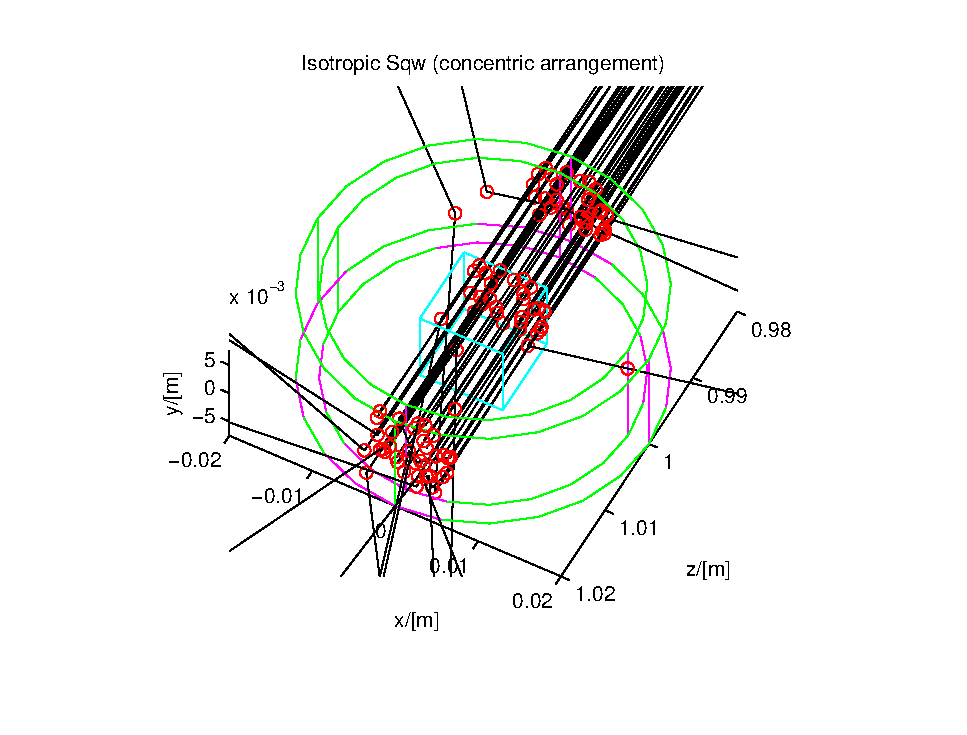
\includegraphics[width=0.9\textwidth]{figures/sqw.eps}
  \end{center}
\caption{An $l-^4$He sample in a cryostat, simulated with the Isotropic\_Sqw component in concentric geometry.}
\label{f:isotropic-sqw}
\end{figure}

The sample component \emph{Isotropic\_Sqw} has been developed in order to simulate neutron scattering from any isotropic material such as liquids, glasses (amorphous systems), polymers and powders (currently, mono-crystals cannot be handled).
The component treats coherent and incoherent neutron scattering and may be used to model most materials, including sample environments with concentric geometries.
The structure and dynamics of isotropic samples can be characterised by the dynamic structure factor $S(q,\omega)$, which determines the interaction between neutrons and the sample and therefore can be used as a probability distribution of $\omega$-energy and $q$-momentum transfers. It handles coherent and incoherent processes, both for elastic and inelastic interactions.
The main input for the component is $S(q,\omega)$ tables, or powder structure files.

Usage examples of this component can be found in the \\
\verb+Neutron site/tests/Test_Isotropic_Sqw+, the \\
\verb+Neutron site/ILL/ILL_H15_IN6+ and the \verb+ILL_TOF_Env+ instruments from the \verb+mcgui+.

\subsection{Neutron interaction with matter - overview}

When a neutron enters a material, according to usual models, it 'sees' atoms as disks with a surface equal to the total cross section of the material $\sigma_{tot}$. The latter includes absorption, coherent and incoherent contributions, which all depend on the incoming neutron energy.
The transmission probability follows an exponential decay law accounting for the total cross section.

For the neutron which is not transmitted, we select a scattering position along the path, taking into account the secondary extinction and absorption probability. In this process, the neutron is considered to be a particle or an attenuated wave.

Once a scattering position has been assigned, the neutron interacts with a material excitation. Here we turn to the wave description of the neutron, which interacts with the whole sample volume. The distribution of excitations, which determines their relative intensity in the scattered beam, is simply the dynamic structure factor - or scattering law - $S(q,\omega)$. We shall build probability distributions from the scattering law in order to improve the efficiency of the method by favoring the $(q,\omega)$ choice towards high $S(q,\omega)$ regions.

The neutron leaves the scattering point when a suitable $(q, \omega)$ choice has been found to satisfy the conservation laws. The method is iterated until the neutron leaves the volume of the material, therefore allowing multiple scattering contributions, which will be considered in more details below.

No experimental method makes it possible to accurately measure the multiple scattering contribution, even though it can become significant at low $q$ transfers (below the first diffraction maximum), where the single scattering coherent signal is weak in most materials. This is why attemps have been made to reduce the multiple scattering contribution by partitioning the sample with absorbing layers. However, this is not always applicable thus makiong the simulation approach very valuable.

The method presented here for handling neutron interaction with isotropic materials is similar in many respects to the earlier MSC \cite{msc}, Discus \cite{discus} and MSCAT \cite{mscat} methods, but the implementation presented here is part of a more general treatment of a sample in an instrument.

\subsection{Theoretical side}

\subsubsection{Pair correlation function $g(r)$ and Dynamic structure factor $S(q,\omega)$}

In the following, we consider an isotropic medium irradiated with a cold or thermal neutron beam. We ignore the possible thermal fission events and assume that the incoming neutron energy does not correspond to a Breit-Wigner resonance in the material. Furthermore, we do not take into account quantum effects in the material, nor refraction and primary extinction.

Following Squires \cite{squires}, the experimental counterpart of the scattering law $S(q,\omega)$ is the neutron double differential scattering cross section for both coherent and incoherent processes:
\begin{equation}\label{eq:d2sigma}
\frac{d^2\sigma}{d\Omega dE_f} = \frac{\sigma}{4\pi}\frac{k_f}{k_i} N S(q, \omega)
\end{equation}
which describes the amount of neutrons scattered per unit solid angle $d\Omega$ and per unit final energy $dE_f$. In this equation, $N=\rho V$ is the number of atoms in the scattering volume $V$ with atomic number density $\rho$, $E_f, E_i, k_f, k_i$ are the kinetic energy and wavevectors of final and initial states respectively, $\sigma$ is the bound atom scattering cross-section, $\Omega$ is the solid angle and $q,\omega$ are the wave-vector and energy transfer at the sample. In practice, the double differential cross section is a linear combinaison of the coherent and incoherent parts as:
\begin{equation}
\label{eq:S=coh+inc}
\sigma S(q,\omega) = \sigma_{coh} S_{coh}(q,\omega) + \sigma_{inc} S_{inc}(q,\omega)
\end{equation}
where the subscripts $coh$ and $inc$ stand for the coherent and incoherent contributions respectively.

We define its norm on a selected $q$ range:
\begin{equation}
|S| = \iint S(q,\omega) dq d\omega .
\end{equation}
The norm $\lim_{q \rightarrow \infty} |S| \simeq q$ for large $q$ values, and can only be defined on a restricted $q$ range.

Some easily measureable coherent quantities in a liquid are the \emph{static pair correlation function} $g(r)$ and the \emph{structure factor} $S(q)$, defined as:
\begin{eqnarray}
\rho g(\vec{r}) &=& \frac{1}{N} \sum_{i=1}^N \sum_{j \neq i} \langle \delta(\vec{r}+\vec{r}_i-\vec{r}_j) \rangle \\
S(\vec{q}) &=&\int S(\vec q,\omega) d\omega \label{eq:sq} \\
           &=&1 + \rho \int_V [g(\vec{r})-1] e^{i\vec{q}.\vec{r}} d\vec{r} \\
           &=&1 + \rho \int_{0}^{\infty} [g(r)-1] \frac{\sin(qr)}{qr} 4 \pi r^2 dr {\rm\ in\ isotropic\ materials.}
\end{eqnarray}
The latter expression, in isotropic materials, may be Fourier transformed as:
\begin{equation}
\label{eq:gr-sq}
g(r)-1 =\frac{1}{2\pi^2 \rho} \int_0^\infty q^2 [S(q) -1] \frac{sin(qr)}{qr} dq
\end{equation}
Both $g(r)$ and $S(q)$ converge to unity for large $r$ and $q$ values respectively, and they are representative of the atoms spatial distribution. In a liquid $\lim_{q \rightarrow 0} S(q) = \rho k_B T \chi_T$ where $\chi_T=(\frac{\partial \rho}{\partial P})_{V,T}$ is the compressibility \cite{Egelstaff67,fischer05}. In perfect gases, $S(q) = 1$ for all $q$. These quantities are obtained experimentally from diffractometers.
In principle, $S_{inc}(q) = 1$ in all materials, but a $q$ dependence is rather usual, partly due to the Debye-Waller factor $e^{-q^2 \langle u^2 \rangle}$. Anyway, $S_{inc}(q)$ converges to unity at high $q$.

The static pair correlation function $g(r)$ is the probability to find a neighbouring atom at a given distance (unitless). Since $g(0) = 0$, Eq. (\ref{eq:gr-sq}) provides a useful normalisation sum-rule for coherent $S(q)$:
\begin{equation}
\label{eq:sq-nomr1}
\int_0^\infty q^2 [S(q) - 1] dq = -2\pi^2\rho {\rm\ for\ coherent\ contribution.}
\end{equation}
This means that the integrated oscillations (around 1) of $S_{coh}(q)$ are directly related to the density of the material $\rho$.
In practice, the function $S(q)$ is often known on a restricted range $q \in [0, q_{max} ]$, due to either limitations in the sample molecular dynamics simulation, or the measurement itself.
In first approximation we consider that Eq. (\ref{eq:sq-nomr1}) can be applied in this range, i.e. we neglect the large $q$ contributions provided $S(q)-1$ converges faster than $1/q^2$. This is usually true after 2-3 oscillations of $S(q)$ in liquids.
Then, in isotropic liquid-like materials, Eq. (\ref{eq:sq-nomr1}) provides a normalisation sum-rule for $S$.

\subsection{Theoretical side - scattering in the sample}

The Eq. \ref{eq:d2sigma} controls the scattering in the whole sample volume.
Its implementation in a propagative Monte Carlo neutron code such as \emph{McStas} can be summarised as follows:
\begin{enumerate}
{\item Compute the propagation path length in the material by geometrical intersections between the neutron trajectory and the sample volume.}
{\item Evaluate the total cross section from the integration of the scattering law over the accessible dynamical range (Section \ref{s:inter-proba}).}
{\item Use the total cross section to determine the probability of interaction for each neutron along the path length, and select a scattering position.}
{\item Weight neutron interaction with the absorption probability and select the type of interaction (coherent or incoherent).}
{\item Select the wave vector and energy transfer from the dynamic structure factor $S(q,\omega)$ used as a probability distribution (Section \ref{s:choose-qw}). Apply the detailed balance.}
{\item Check whether selection rules can be solved (Section \ref{s:rules-qw}). If they cannot, repeat (5).}
\end{enumerate}
This procedure is iterated until the neutron leaves the sample. We shall now detail the key steps of this implementation.

\subsubsection{Evaluating the cross sections and interaction probability}
\label{s:inter-proba}

Following Sears \cite{Sears75}, the total scattering cross section for incoming neutrons with initial energy $E_i$ is
\begin{equation}
\label{eq:iisigma}
\sigma_s(E_i) = \iint \frac{d^2 \sigma}{d\Omega dE_f} d\Omega dE_f = \frac{N \sigma}{4\pi} \iint \frac{k_f}{k_i} S(q, \omega) d\Omega dE_f
\end{equation}
where the integration runs over the entire space and all final neutron energies.
As the dynamic structure factor is defined in the $q,\omega$ space, the integration requires a variable change. Using the momentum conservation law and the solid angle relation $\Omega=2\pi(1-cos \theta)$, were $\theta$ is the solid angle opening, we draw:
\begin{equation}
\label{eq:iqSqw}
\sigma_s(E_i) = N \iint \frac{\sigma S(q,\omega) q}{2 k_i^2} dq d\omega.
\end{equation}
This integration runs over the whole accessible $q,\omega$ dynamical range for each incoming neutron.
In practice, the knowledge of the dynamic structure factor is defined over a limited area with $q \in [q_{min}, q_{max}]$ and $\omega \in [\omega_{min}, \omega_{max}]$ which is constrained by the method for obtaining $S(q,\omega)$, i.e. from previous experiments, molecular dynamics simulations, and analytical models. It is desirable that this area be as large as possible, starting from 0 for both ranges. If we use $\omega_{min} \rightarrow 0$, $q_{min} \rightarrow 0$, $\omega_{max} > 4E_i$ and $q_{max} > 2k_i$, we completely describe all scattering processes for incoming neutrons with wavevector $k_i$ \cite{msc}.

This means that in order to correctly estimate the total intensity and multiple scattering, the knowledge of $S(q,\omega)$ must be wider (at least twice in $q$, as stated previously) than the measurable range in the corresponding experiment.
As a side effect, a self consistent iterative method for finding the true scattering law from the measurement itself is not theorically feasible, except for providing crude approximations.
However, that measured dynamic structure factor may be used to estimate the multiple scattering for a further measurement using longer wavelength neutrons.
In that case, extrapolating the scattering law beyond the accessible measurement ranges might improve substantially the accuracy of the method, but this discussion is beyond the scope of this paper.

Consequently, limiting the $q$ integration in Eq. \ref{eq:iqSqw} to the maximum momentum transfer for elastic processes $2 k_i$, we write the total scattering cross section as
\begin{equation}
\label{eq:iqSq}
\sigma_s(E_i) \simeq \frac{N}{2 k_i^2} \int_0^{2k_i} q \sigma S(q) dq.
\end{equation}
Using Eq. \ref{eq:S=coh+inc}, it is possible to define similar expressions for the coherent and incoherent terms $\sigma_{coh}(E_i)$ and $\sigma_{inc}(E_i)$ respectively. These integrated cross sections are usually quite different from the tabulated values \cite{ILLblue} since the latter are bound scattering cross sections.

Except for a few materials with absorption resonances in the cold-thermal energy range, the absorption cross section for an incoming neutron of velocity $v_i=\sqrt{2E_i/m}$, where $m$ is the neutron mass, is computed as
$\sigma_{abs}(E_i) = \sigma_{abs}^{{\rm 2200}}\frac{2200 m/s}{\sqrt{2E_i/m}}$, where $\sigma_{abs}^{{\rm 2200}}$ is obtained from the literature \cite{ILLblue}.

We now determine the total cross section accounting for both scattering and absorption
\begin{equation}
\sigma_{tot}(E_i) = \sigma_{abs}(E_i) + \sigma_s(Ei).
\end{equation}
The neutron trajectory intersection with the sample geometry provides the total path length in the sample $d_{exit}$ to the exit.
Defining the linear attenuation $\mu(E_i) = \rho\sigma_{tot}(E_i)$, the probability that the neutron event is transmitted along path $d_{exit}$ is $e^{-\mu(E_i) d_{exit}}$.

If the neutron event is transmitted, it leaves the sample. In previous Monte Carlo codes such as DISCUSS \cite{discus}, MSC \cite{msc} and MSCAT \cite{mscat}, each neutron event is forced to scatter to the detector area in order to improve the sample scattering simulation statistics and reduce the computing time. The corresponding instrument model is limited to a neutron event source, a sample and a detector. It is equaly possible in the current implementation to 'force' neutron events to scatter by applying a correction factor $\pi_0=1-e^{-\mu(E_i) d_{exit}}$ to the neutron statistical weight. However, the \emph{McStas} instrument model is often build from a large sequence of components. Eventhough the instrument description starts as well with a neutron event source, more than one sample may be encountered in the course of the neutron propagation and multiple detectors may be positioned anywhere in space, as well as other instrument components (e.g. neutron optics). This implies that neutron events scattered from a sample volume should not focus to a single area.  Indeed, transmitted events may reach other scattering materials and it is not desirable to force all neutron events to scatter. The correction factor $\pi_0$ is then not applied, and neutron events can be transmitted through the sample volume. The simulation efficiency for the scattering then drops significantly, but enables to model much more complex arrangements such as concentric sample environments, magnets and monochromator mechanical parts, and neutron filters.

If the neutron is not transmitted, the neutron statistical weight is multiplied by a factor
\begin{equation}
\pi_1 = \frac{\sigma_s(E_i)}{\sigma_{tot}(E_i)}
\end{equation}
to account for the fraction of absorbed neutrons along the path, and we may in the following treat the event as a scattering event.
Additionally, the type of interaction (coherent or incoherent) is chosen randomly with fractions $\sigma_{coh}(E_i)$ and $\sigma_{inc}(E_i)$.

The position of the neutron scattering event along the neutron trajectory length $d_{exit}$ is determined by \cite{Mildner77,discus}
\begin{equation}
d_{s} = -\frac{1}{\mu(E_i)} \ln(1 - \xi[1 -e^{-\mu(E_i) d_{exit}}])
\end{equation}
where $\xi$ is a random number in [0,1]. This expression takes into account secondary extinction, originating from the decrease of the beam intensity through the sample (self shielding).

\subsubsection{Choosing the $q$ and $\omega$ transfer from $S(q, \omega)$ }
\label{s:choose-qw}

The choice of the $(q, \omega)$ wavevector-energy transfer pair could be done randomly, as in the first event of the second order scattering evaluation in DISCUS \cite{discus}, but it is somewhat inefficient except for materials showing a broad quasi-elastic signal. As the scattering originates from structural peaks and excitations in the material $S(q, \omega)$, it is usual \cite{mscat} to adopt an importance sampling scheme by focusing the $(q, \omega)$ choice to areas where the intensity of $S(q, \omega)$ is high. In practice, this means that the neutron event should scatter preferably on e.g. Bragg peaks, quasielastic contribution and phonons.

The main idea to implement the scattering from $S(q, \omega)$ is to cast two consecutive Monte Carlo choices, using probability distribution built from the dynamic structure factor.
We define first the probability $P_{\omega}(\omega)$ as the \emph{unweighted} fraction of modes whose energy lies between $\omega$ and $\omega+d\omega$
\begin{equation}
P_{\omega}(\omega) d\omega = \frac{\int_0^{q_{max}} q S(q,\omega) dq}{|S|},
\end{equation}
where $|S| = \iint S(q,\omega) dq d\omega$ is the norm of $S(q,\omega)$ in the available dynamical range $q \in [q_{min}, q_{max}]$ and $\omega \in [\omega_{min}, \omega_{max}]$.
The probability $P_{\omega}(\omega)$ is normalised to unity, $\int P_{\omega}(\omega) d\omega = 1$, and is a probability distribution of mode energies in the material. We then choose randomly an energy transfer $\omega$ from this distribution.

Similarly, in order to focus the wavevector transfer choice, we define the probability distribution of wavevector $P_q(q\mid\omega)$ for the selected energy transfer lying between $\omega$ and $\omega+d\omega$
\begin{equation}
P_q(q\mid\omega) = \frac{q S(q, \omega)}{S(q)},
\end{equation}
from which we choose randomly a wavevector transfer $q$, knowing the energy transfer $\omega$.
These two probability distributions extracted from $S(q,\omega)$ are shown in Fig. \ref{f:isotropic-sqw-proba}, for a model $S(q,\omega)$ function built from the {\it l}-$^4$He elementary excitation (Data from Donnelly).

\begin{figure}
  \begin{center}
    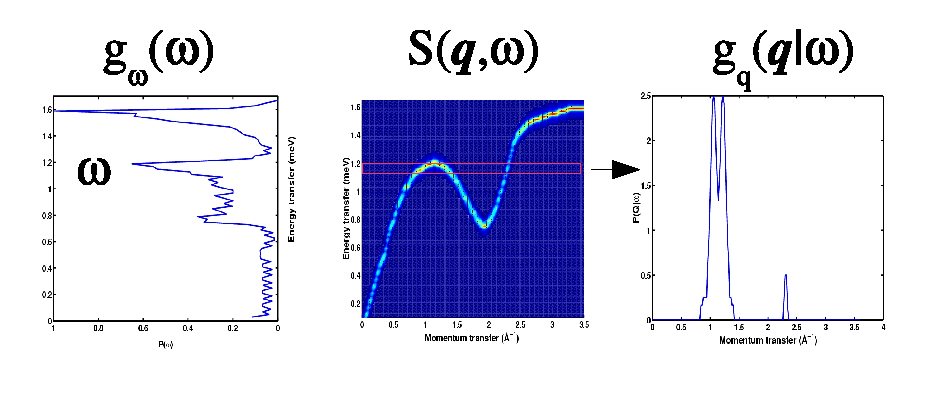
\includegraphics[width=0.9\textwidth]{figures/Sqw_sampling.eps}
  \end{center}
\caption{\emph{Centre}: Model of dynamic structure factor $S(q,\omega)$ for l-$^4$He ; \emph{left}: probability distribution $g_\omega$ (horizontal axis) of energy transfers (vertical axis, density of states) ; \emph{right} : probability distribution $g_q(\omega)$ (vertical axis) of momentum transfers (horizontal axis) for a given energy transfer $\hbar \omega \sim 1.1$ meV.}
\label{f:isotropic-sqw-proba}
\end{figure}

Then a selection between energy gain and loss is performed with the detailed balance ratio $e^{-\hbar \omega / k_B T}$. In the case of Stokes processes, the neutron can not loose more than its own energy to the sample dynamics, so that $\hbar \omega < E_i$. This condition breaks the symmetry between up-scattering and down-scattering.

\subsubsection{Solving selection rules and choosing the scattered wave vector}
\label{s:rules-qw}

The next step is to check that the conservation laws
\begin{eqnarray}
\hbar \omega &=& E_i - E_f = \frac{\hbar^2}{2m}(k_i^2 - k_f^2) \label{eq:sqw-w-transfer} \\
\vec q &=& \vec k_i - \vec k_f \label{eq:sqw-q-transfer}
\end{eqnarray}
can be satisfied. These conditions are closely related to the method for selecting the outgoing wave vector direction.

When the final wave vector has to be computed, the quantities $\vec{k}_i$, $\hbar \omega$ and $q = |\vec{q}|$ are known.
We solve the energy conservation law Eq. (\ref{eq:sqw-w-transfer}) and we select randomly $k_f$ as one of the two roots.

The scattering angle $\theta$ from the initial $k_i$ direction is determined from the momentum conservation law $cos(\theta) = (k_i^2 + k_f^2 - q^2)/(2k_i k_f)$, which defines a scattering cone. We then choose randomly a direction on the cone.

If the selection rules can not be verified (namely $|cos(\theta)| > 1$), a new $(q,\omega)$ random choice is performed (see Section \ref{s:choose-qw}).
It might appear inefficient to select the energy and momentum tranfers first and check the selection rules afterwards. However, in practice, the number of iterations to actually scatter on a high probability process and satisfy these rules is limited, usually below 10. Moreover, as these two steps are simple, the whole process requires a limited number of computer operations.

As mentioned in Section \ref{s:inter-proba}, previous multiple scattering estimation codes \cite{msc,mscat,discus} force the outgoing neutron event to come into the detector area and time window, thus improving dramatically the code efficiency. This choice sets the measurable energy and momentum transfers for the last scattering event in the sample, so that the choice of the scattering excitation actually requires a more complex sampling mechanism for the dynamic structure factor. As the present implementation makes no assumption on the simulated instrument part which is behind the sample, we can not apply this method. Consequently, the efficiency of the sample scattering code is certainly lower than previous codes, but on the other hand it does not depend on the type of instrument simulation. In particular, it may be used to model any material in the course of the neutron propagation along the instrument model (filters, mechanical parts, samples, shields, radiation protections).

Once the scattering probability and position, the energy and momentum transfers and the neutron momentum after scattering have all been defined, the whole process is iterated until the neutron is transmitted and exits the sample volume.

\subsubsection{Extension to powder elastic scattering}

In principle, the component can work in purely elastic mode if only the $\omega = 0$ column is available in $S$.
Anyway, in the diffractionists world, people do not usually define scattering with $S(q)$ (Eq. \ref{eq:sq}), but through the scattering vector $\boldsymbol{\tau}$, multiplicity $z(\tau)$ (for powders), and $|F^2|$ structure factors including Debye-Waller factors, as in Eq. \ref{eq:sigma_coh_el}.

When doing diffraction, and neglecting inelastic contribution as first approximation, we may integrate Eq. \ref{eq:d2sigma}, keeping $k_i = k_f$.
\begin{eqnarray}
\left(\frac{d\sigma}{d\Omega}\right)_{\rm coh.el.}(|q|) &=& \int_0^\infty \frac{d^2\sigma_{coh}}{d\Omega dE_f} dE_f = \frac{N \sigma_{coh}}{4\pi} S_{coh}(q) \\
& = & N\frac{(2\pi)^3}{V_0}\sum_{\boldsymbol{\tau}} \delta(\boldsymbol{\tau} - \boldsymbol{q})|F_{\boldsymbol{\tau}}|^2 {\rm\ from\ Eq.\ (\ref{eq:sigma_coh_el})}
\end{eqnarray}
with $V_0 = 1/\rho$ being the volume of a lattice unit cell. Then we come to the formal equivalence, in the powder case \cite{squires} (integration over Debye-Scherrer cones):
\begin{eqnarray}\label{eq:sq-F2}
S_{coh}(q) = \frac{\pi \rho}{2\sigma_{coh}} \frac{z(q)}{q^2} |F_q|^2 {\rm\ in\ a\ powder.}
\end{eqnarray}
for each lattice Bragg peak wave vector $q$.
The normalisation rule Eq. (\ref{eq:sq-nomr1}) can not usually be applied for powders, as the $S(q)$ is a set of Dirac peaks for which the $\int q^2 S(q) dq$ is difficult to compute, and $S(q)$ does not converge to unity for large $q$. Each $F^2$ Dirac contribution may be broaden when specifiying a diffraction peak width.

Of course, the component PowderN (see section \ref{powder}) can handle powder samples efficiently (faster, better accuracy), but does not take into account multiple scattering, nor secondary extinction (which is significant for materials with large absorption cross sections). On the other side, the current Isotropic\_Sqw component assumes a powder packing factor of 1 (massive sample). To change into a lower packing factor, use a lower powder density.

\subsubsection{Important remarks and limitations}

Since the choice of the interaction type, we know that the neutron \emph{must} scatter, with an appropriate $\vec k_f$ outgoing wave vector. If any of the choices in the method fails:
\begin{enumerate}
\item the two roots $k_f^+$ and $k_f^-$ are imaginary, which means that conservation laws can not be satisfied and for instance the selected energy transfer is higher than the incoming neutron energy
\item the radius of the target circle is imaginary, that is $|cos(\theta)| > 1$.
\end{enumerate}
then a new $(q, \omega)$ set is drawn, and the process is iterated until success or - at last - removal of the neutron event. These latter absorptions are then reported at the end of the simulation, as it never occurs in reality - neutrons that scatter do find a suitable $(q, \omega)$ set.\index{Removed neutron events}

The $S(q,\omega)$ data sets should be as wide a possible in $q$ and $\omega$ range, else scattering conditions will be limited by the reduced data set (specially multiple scattering estimates). On the other hand, when $q$ and $\omega$ ranges are too large, some Monte Carlo choices lead to scattering temptatives in non useful regions of $S$, which reduces dramatically the algorithm efficiency.

The best settings are:
\begin{enumerate}
\item to have the widest $q$ and $\omega$ range for $S(q,\omega)$ data sets,
\item to either set $wmax$ and $qmax$ to the maximum scatterable energy and wavevectors,
\item or alternatively request the automatic range optimisation by setting parameter \verb+auto_qw=1+. This is recommended, but may sometimes miss a few neutrons if the $q,\omega$ beam range has been guessed too small.
\end{enumerate}

Focusing the $q$ and $\omega$ range (e.g. with 'auto\_qw=1'), to the one being able to scatter the incoming beam, when using the component does improve significantly the speed of the computation. Additionally, if you restrict the scattering to the first order only (parameter 'order=1'), then you may specify the angular vertical extension $d\phi$ of the scattering area to gain optimised focusing. This option does not apply when handling multiple scattering (which emits in $4\pi$ many times before exiting the sample).

A bilinear interpolation for the $q,\omega$ determination is used to improve the accuracy on the scattered intensity, but it may be unactivated when setting parameter \verb+interpolate=0+. This will often result in a discrete $q,\omega$ sampling.

As indicated in the previous section, the Isotropic\_Sqw component is not as efficient as PowderN for powder single scattering, but handles scattering processes in a more accurate way (secondary extinction, multiple scattering).

\subsection{The implementation}

\begin{table}
  \begin{center}
  {\let\my=\\
    \begin{tabular}{|lr|p{0.6\textwidth}|}
    \hline
Parameter & type & meaning \\
    \hline
Sqw\_coh   & string              & Coherent scattering data file name. Use 0, NULL or "" to disable  \\
Sqw\_inc   & string              & Incoherent scattering data file name. Use 0, NULL or "" to scatter isotropically (Vanadium like)  \\
sigma\_coh & [barns]      & Coherent scattering cross-section. -1 to disable \\
sigma\_inc & [barns]      & Incoherent scattering cross-section. -1 to disable \\
sigma\_abs & [barns]      & Absorption cross-section. -1 to disable  \\
V\_rho     & [\AA$^{-3}$] & atomic number density. May also be specified with molar weight \emph{weight} in [g/mol] and material \emph{density} in [g/cm$^3$] \\
T          & [K]          & Temperature. 0 disables detailed balance \\
    \hline
xwidth   & [m] & \\
yheight  & [m] & dimensions of a box shaped geometry \\
zdepth   & [m] & \\
radius\_o & [m] & dimensions of a cylinder shaped geometry  \\
radius\_i & [m] & sphere geometry if radius\_i=0  \\
thickness& [m] & thickness of hollow shape  \\
    \hline
auto\_qw  & boolean & Automatically optimise probability tables during simulation  \\
auto\_norm& scalar  & Normalize $S(q,\omega)$ when -1, use raw data when 0, multiply $S$ by given value when positive \\
%interpolate & boolean & Smooth $S(q,\omega)$ table (recommended) \\
order     & integer & Limit multiple scattering up to given order. 0 means all orders  \\
concentric& boolean & Enables to 'enter' inside concentric hollow geometries  \\
    \hline
    \end{tabular}
    \caption{Main Isotropic\_Sqw component parameters}
    \label{t:sqw-param}
  }
  \end{center}
\end{table}

\subsubsection{Geometry}

The geometry for the component may be box, cylinder and sphere shaped, either filled or hollow. Relevant parameters for this purpose are as follow:
\begin{itemize}
\item {\bf box}: dimensions are $x_{width} \times y_{height} \times z_{depth}$.
\item {\bf box, hollow}: \emph{idem}, and the side wall thickness is set with $thickness$.
\item {\bf cylinder}: dimensions are $r$ for the radius and $y_{height}$ for the height.
\item {\bf cylinder, hollow}: \emph{idem}, and hollow part is set with $thickness$.
\item {\bf sphere}: dimension is $r$ for the radius.
\item {\bf sphere, hollow}: \emph{idem}, and hollow part is set with $thickness$.
\end{itemize}
The AT position corresponds to the centre of the sample.

Hollow shapes are particularly useful to model complex sample environments. Refer to the dedicated section below for more details on this topic.

\subsubsection{Dynamical structure factor}

The material behaviour is specified through the total scattering cross-sections $\sigma_{coh}$, $\sigma_{inc}$, $\sigma_{abs}$, and the $S(q, \omega)$ data files.

If you are lucky enough to have access to separated coherent and incoherent contributions (e.g. from material simulation), simply set Sqw\_coh and Sqw\_inc parameter to the files names. If on the other hand you have access to a global data set containing incoherent scattering as well (e.g. the result of a previous experiment), use Sqw\_coh parameter, set the $\sigma_{coh}$ parameter to the sum of both contributions $\sigma_{coh}+\sigma_{inc}$, and set $\sigma_{inc}=-1$. This way we only use one of the two implemented  scattering channels. Such global data sets may originate from previous experiments, as far as you have applied all known corrections (multiple scattering, geometry, ...).

In any case, the accuracy of the $S(q, \omega)$ data limits the $q$ and $\omega$ resolution of the simulation, eventhough a bilinear interpolation is performed in order to smooth binning. The sampling of data files should then be as thin as possible.

If the Sqw\_inc parameter is left unset but the $\sigma_{inc}$ is \emph{not} zero, an isotropic incoherent elastic scattering is used, just like the V\_sample component (see section \ref{s:v_sample}).

Anyway, as explained below, it is also possible to simulate the elastic scattering from a powder file (see below).

\subsubsection{File formats: $S(q,\omega)$ inelastic scattering}

The format of the data files is free text, consisting of three numerical blocks, separated by empty lines or comments, in the following order
\begin{enumerate}
\item A vector of length $m$ containing wavevector $q$ values, in \AA$^{-1}$.
\item A vector of length $n$ containing energy $\omega$ values, in meV.
\item A matrix of size $m$ rows by $n$ columns, of $S(q, \omega)$ values, in meV$^{-1}$.
\end{enumerate}
Any line beginning with any character of \verb+#;/%+ is considered to be a comment, and lines which can not be read as vectors/matrices are ignored.

The file header may optionally contain parameter settings for the material, as comments, with keywords as in the following example:
\begin{verbatim}
  #V_0         35   cell volume [Angs^3]
  #V_rho       0.07 atom number density [at/Angs^3]
  #sigma_abs   5    absorption cross section [barns]
  #sigma_inc   4.8  incoherent cross section [barns]
  #sigma_coh   1    coherent cross section  [barns]
  #Temperature 10   for detailed balance [K]
  #density     1    material density [g/cm^3]
  #weight      18   material molar weight [g/mol]
  #nb_atoms    6    number of atoms per unit cell
\end{verbatim}
Some \verb+sqw+ data files are included in the \MCS\ distribution data directory, and they contain material parameter settings in their header, so that you may use:
\begin{verbatim}
Isotropic_Sqw(<geometry parameters>, Sqw_coh="He4_liq_coh.sqw", T=4)
\end{verbatim}

Example files are listed as \verb+*.sqw+ files in directory \verb+MCSTAS/data+. A table of $S(q,\omega)$ data files for a few liquids are listed in Table \ref{t:liquids-data} (page \pageref{t:liquids-data}).

\subsubsection{File formats: $S(q)$ liquids}

This file format provides a mean to import directly an $S(q)$ data set, when setting parameters:
\begin{verbatim}
  powder_format=qSq
\end{verbatim}
The 'Sqw\_coh' (or 'Sqw\_inc') file should contains a single numerical block, which column assignment is defaulted as $q$ and $S(q)$ being the first and second column respectively. This may be overridden from the file header with '\#column' keywords, as in the example:
\begin{verbatim}
  #column_q  2
  #column_Sq 1
\end{verbatim}
Such files can only handle elastic scattering.

\subsubsection{File formats: powder structures (LAZY, Fullprof, Crystallographica)}

Data files as used by the component PowderN may also be read. Data files of type \verb'lau' and \verb'laz' in the \MCS\ distribution data directory are self-documented in their header. They do not need any additional parameters to be used, as in the example:
\begin{verbatim}
  Isotropic_Sqw(<geometry parameters>, Sqw_coh="Al.laz")
\end{verbatim}
Other column-based file formats may also be imported e.g. with parameters such as:
\begin{verbatim}
  powder_format=Crystallographica
  powder_format=Fullprof
  powder_Dd    =0
  powder_DW    =1
\end{verbatim}
The last two parameters may as well be specified in the data file header with lines:
\begin{verbatim}
  #Debye_Waller 1
  #Delta_d/d    1e-3
\end{verbatim}
The powder description is then translated into $S(q)$ by using Eq. (\ref{eq:sq-F2}).
In this case, the density $\rho = n/V_0$ is the number of atoms in the inverse volume of the unit cell.

As the component builds an $S(q)$ from the powder structure description, the accuracy of the Isotropic\_Sqw component is limited by the binning during that conversion. This is usually enough to describe sample environments including powders (aluminium, copper, ...), but it is recommended to rather use PowderN for faster and accurate powder diffraction, eventthough this latter does not implement multiple scattering.

Such files can only handle elastic scattering. A list of common powder definition files is available in Table \ref{t:powders-data} (page \pageref{t:powders-data}).

\subsubsection{Concentric geometries, sample environment}
\index{Sample environments}

The component has been designed in a way which enables to describe complex imbricated set-ups, i.e. what you need to simulate sample environments. To do so, one has first to use hollow shapes, then keep in mind that each surrounding geometry should be first declared before the central position (usually the sample) with the \verb+concentric=1+ parameter, but also duplicated (with an other instance name) at a symmetric position with regards to the centre as in the example (shown in Fig. \ref{f:isotropic-sqw}):
\begin{verbatim}
COMPONENT s_in=Isotropic_Sqw(
  thickness=0.001, radius=0.02, yheight=0.015,
  Sqw_coh="Al.laz", concentric=1)
AT (0,0,1) RELATIVE a

COMPONENT sample=Isotropic_Sqw(
  xwidth=0.01, yheight=0.01, zdepth=0.01,
  Sqw_coh="Rb_liq_coh.sqw")
AT (0,0,1) RELATIVE a

COMPONENT s_out=Isotropic_Sqw(
  thickness=0.001, radius=0.02, yheight=0.015,
  Sqw_coh="Al.laz")
AT (0,0,1) RELATIVE a
\end{verbatim}
Central component may be of any type, not specifically an Isotropic\_Sqw instance. It could be for instance a Single\_crystal or a PowderN.
In principle, the number of surrounding shells is not restricted.
The only restriction is that neutrons that scatter (in $4\pi$) can not come back in the instrument description, so that some of the multiple scattering events are lost. Namely, in the previous example, neutrons scattered by the outer wall of the cryostat \verb+s_out+ can not come back to the sample or to the other cryostat wall \verb+s_in+. As these neutrons have usually few chances to reach the rest of the simulation, we expect that the approximation is fair.

\subsection{Validation}
For constant incoherent scattering mode, V\_sample, PowderN, Single\_crystal and Isotropic\_Sqw produce equivalent results, eventhough the two later are more accurate (geometry, multiple scattering). Execution times are equivalent.

Compared with the PowderN component, the $S(q)$ method is twice slower in computation time, and intensity is usually lower by typically 20 \% (depending on scattering cross sections), the difference arising from multiple scattering and secondary extinction (not handled in PowderN). The PowderN component is intrinsically more accurate in $q$ as each Bragg peak is handled separately as an exact Dirac peak, with optional $\Delta q$ spreading. In Isotropic\_Sqw, an approximated $S(q)$ table is built from the $F^2$ data, and is coarser. Still, differences in the diffraction pattern are limited.

The Isotropic\_Sqw component has been benchmarked against real experiment for liquid Rubidium (Copley, 1974) and liquid Cesium (Bodensteiner  and Dorner, 1989), and the agreement is excellent.

The \verb+Test_Isotropic_Sqw+ test/example instrument exists in the distribution for this component.




